
\documentclass[a4paper,8pt]{extarticle} % extarticle allows to use font size of 8pt.

\usepackage[a4paper, top=1.6cm, bottom=2cm, left=1.6cm, right=1.6cm]{geometry} % Marge reduction.

\usepackage{ifxetex}

\ifxetex
  \usepackage{fontspec}
  \defaultfontfeatures{Ligatures=TeX} % To support LaTeX quoting style
  \setmainfont{Casablanca Antique}
\else
	\usepackage[T1]{fontenc} 		% Font encoding.
	\usepackage[utf8]{inputenc} 	% Document encoding.
	\usepackage{palatino} 			% Font.
\fi

\usepackage{microtype}			% Greatly improves general appearance of the text.
\usepackage{SIunits}			% Unit appearance.
\usepackage{array}				% Additionnal options for arrays.
\usepackage{colortbl}			% Additionnal options for coloring arrays.
\usepackage{multicol}			% Allows to divide a part of the page in multiple columns.
\usepackage{framed}				% Boxes.
\usepackage[inline]{enumitem}   % Display inline lists.
\usepackage{etoolbox}           % General utility. Good for lists for instance.
\usepackage{newfloat}			% Used to create new flottable environnements.
	\DeclareFloatingEnvironment[placement=htbp!]{unitframeFlot}
\usepackage{keyval}             % Used to create maps of commands/labels/objects.
	\makeatletter                  % Mandatory for the usage of keyval.
\usepackage{xstring}            % String parsing, cutting, etc.
\usepackage{xparse}             % List utilities.
\usepackage{xspace}				% Define commands that appear not to eat spaces.
\usepackage{textcomp} 			% for the straight single quote \textquotesingle.
\usepackage[colorlinks=true]{hyperref} % Links in PDF.
\usepackage[framemethod=TikZ]{mdframed}% For fancy frames.
\usepackage{tikz}				% For fancy frames.

%%% Language specific stuff

% \usepackage[french]{babel}

\frenchbsetup{StandardLists=true} % Necessary to use enumitem with babel/french.

% This has to disappear.

\newcommand{\pouce}{\inch}
\newcommand{\pied}{\foot}
\newcommand{\portee}{\range}

% Labels

\newcommand{\labels@range}{Portée}
\newcommand{\labels@profile}{Profil}
\newcommand{\labels@M}{M}
\newcommand{\labels@WS}{CC}
\newcommand{\labels@BS}{CT}
\newcommand{\labels@S}{F}
\newcommand{\labels@T}{E}
\newcommand{\labels@W}{PV}
\newcommand{\labels@I}{I}
\newcommand{\labels@A}{A}
\newcommand{\labels@Ld}{Cd}
\newcommand{\labels@unitsize}{Taille de l'unité}
\newcommand{\labels@basesize}{Taille du socle}
\newcommand{\labels@trooptype}{Type de troupe}
\newcommand{\labels@specialrules}{Règles spéciales}
\newcommand{\labels@equipment}{Équipement}
\newcommand{\labels@options}{Options}
\newcommand{\labels@commandgroup}{État-Major}
\newcommand{\labels@lords}{Seigneurs}
\newcommand{\labels@heroes}{Héros}
\newcommand{\labels@baseunits}{Unités de base}
\newcommand{\labels@specialunits}{Unités spéciales}
\newcommand{\labels@rareunits}{Unités rares}
\newcommand{\labels@mounts}{Montures}
\newcommand{\labels@specialequipment}{Équipement spécial}
\newcommand{\labels@fantasybattles}{Batailles Fantastiques}
\newcommand{\labels@NinthAge}{Le 9\ieme Âge}
\newcommand{\labels@creators}{Une collaboration des créateurs de l'ETC et du Swedish Comp System}
\newcommand{\labels@latexcredit}{Document réalisé à l'aide de \LaTeX .}

\newcommand{\labels@point}{pt}
\newcommand{\labels@points}{pts}

\newcommand{\labels@armyspecialrules}{Règles spéciales de l'armée}
\newcommand{\labels@armoury}{Armurerie}
\newcommand{\labels@magicitems}{Objets magiques}

% Technical

\newcommand{\free}{gratuit}
\newcommand{\upto}{jusqu'à}
\newcommand{\unlimited}{sans limite de pts}
\newcommand{\permodel}{/fig.}

% Special rules

\newcommand{\ambush}{\specialrule{Embuscade}\xspace}
\newcommand{\armourpiercing}[1]{\specialrule{Perforant\ifblank{#1}{}{~(#1)}}\xspace}
\newcommand{\blurry}{\specialrule{Camouflé}\xspace}
\newcommand{\bodyguard}[1]{\specialrule{Garde du Corps\ifblank{#1}{}{~(#1)}}\xspace}
\newcommand{\breathweapon}[1]{\specialrule{Attaque de Souffle\ifblank{#1}{}{ (#1)}}\xspace}
\newcommand{\channel}{\specialrule{Canalisation}\xspace}
\newcommand{\crushattack}{\specialrule{Attaque Écrasante}\xspace}
\newcommand{\devastatingcharge}{\specialrule{Charge Dévastatrice}\xspace}
\newcommand{\distracting}{\specialrule{Distrayant}\xspace}
\newcommand{\engineer}{\specialrule{Ingénieur}\xspace}
\newcommand{\ethereal}{\specialrule{Éthéré}\xspace}
\newcommand{\fastcavalry}{\specialrule{Cavalerie Légère}\xspace}
\newcommand{\fear}{\specialrule{Peur}\xspace}
\newcommand{\fightinextrarank}{\specialrule{Combat avec un Rang Supplémentaire}\xspace}
\newcommand{\fireborn}{\specialrule{Né du Feu}\xspace}
\newcommand{\flamingattacks}{\specialrule{Attaques Enflammées}\xspace}
\newcommand{\flammable}{\specialrule{Inflammable}\xspace}
\newcommand{\freereform}{\specialrule{Reformation Gratuite}\xspace}
\newcommand{\frenzy}{\specialrule{Frénésie}\xspace}
\newcommand{\fly}[1]{\specialrule{Vol\ifblank{#1}{}{~(#1)}}\xspace}
\newcommand{\grindingattacks}[1]{\specialrule{Attaques de Broyage\ifblank{#1}{}{~(#1)}}\xspace}
\newcommand{\hatred}{\specialrule{Haine}\xspace}
\newcommand{\hellfire}{\specialrule{Flammes de l'Enfer}\xspace}
\newcommand{\hidden}{\specialrule{Caché}\xspace}
\newcommand{\holyattacks}{\specialrule{Attaques Sacrées}\xspace}
\newcommand{\immunetopsychology}{\specialrule{Immunisé à la Psychologie}\xspace}
\newcommand{\impacthits}[1]{\specialrule{Touches d'Impact\ifblank{#1}{}{~(#1)}}\xspace}
\newcommand{\insignificant}{\specialrule{Insignifiant}\xspace}
\newcommand{\largetarget}{\specialrule{Grande Cible}\xspace}
\newcommand{\lethalstrike}{\specialrule{Coup Fatal}\xspace}
\newcommand{\lightningattacks}{\specialrule{Attaques Foudroyantes}\xspace}
\newcommand{\lightningreflexes}{\specialrule{Réflexes Foudroyants}\xspace}
\newcommand{\magicresistance}[1]{\specialrule{Résistance à la Magie\ifblank{#1}{}{~(#1)}}\xspace}
\newcommand{\magicalattacks}{\specialrule{Attaques Magiques}\xspace}
\newcommand{\metalshifting}{\specialrule{Fusion du Métal}\xspace}
\newcommand{\moveorfire}{\specialrule{Mouvement ou Tir}\xspace}
\newcommand{\multipleshots}[1]{\specialrule{Tirs Multiples\ifblank{#1}{}{ (#1)}}\xspace}
\newcommand{\multiplewounds}[2]{\specialrule{Blessures Multi\-ples\ifblank{#1}{}{ (#1\ifblank{#2}{)}{, #2)}}\xspace}}
\newcommand{\notaleader}{\specialrule{Pas un Meneur}\xspace}
\newcommand{\otherworldly}{\specialrule{D'Outre-Monde}\xspace}
\newcommand{\pathmaster}[1]{\specialrule{Maître de la Discipline\ifblank{#1}{}{ (#1)}}\xspace}
\newcommand{\poisonedattacks}{\specialrule{Attaques Empoisonnées}\xspace}
\newcommand{\quicktofire}{\specialrule{Tir Rapide}\xspace}
\newcommand{\randommovement}[1]{\specialrule{Mouvement Aléatoire\ifblank{#1}{}{~(#1)}}\xspace}
\newcommand{\randomattacks}[1]{\specialrule{Attaques Aléatoires\ifblank{#1}{}{~(#1)}}\xspace}
\newcommand{\regeneration}[1]{\specialrule{Régénération\ifblank{#1}{}{ (#1+)}}\xspace}
\newcommand{\requirestwohands}{\specialrule{Arme à deux Mains}\xspace}
\newcommand{\scythes}{\specialrule{Faux}\xspace}
\newcommand{\scout}{\specialrule{Éclaireur}\xspace}
\newcommand{\scouts}{\specialrule{Éclaireurs}\xspace}
\newcommand{\slowtofire}{\specialrule{Tir Lent}\xspace}
\newcommand{\stomp}[1]{\specialrule{Piétinement\ifblank{#1}{}{~(#1)}}\xspace}
\newcommand{\strider}[1]{\specialrule{Guide\ifblank{#1}{}{~(#1)}}\xspace}
\newcommand{\stubborn}{\specialrule{Tenace}\xspace}
\newcommand{\stupidity}{\specialrule{Stupide}\xspace}
\newcommand{\skirmisher}{\specialrule{Tirailleur}\xspace}
\newcommand{\skirmishers}{\specialrule{Tirailleurs}\xspace}
\newcommand{\swiftstride}{\specialrule{Rapide}\xspace}
\newcommand{\thunderouscharge}{\specialrule{Charge Tonitruante}\xspace}
\newcommand{\terror}{\specialrule{Terreur}\xspace}
\newcommand{\toxicattacks}{\specialrule{Attaques Toxiques}\xspace}
\newcommand{\unbreakable}{\specialrule{Indémoralisable}\xspace}
\newcommand{\undead}{\specialrule{Mort-Vivant}\xspace}
\newcommand{\unstable}{\specialrule{Instable}\xspace}
\newcommand{\unwieldy}{\specialrule{Encombrant}\xspace}
\newcommand{\vanguard}{\specialrule{Avant-Garde}\xspace}
\newcommand{\volleyfire}{\specialrule{Tir de Volée}\xspace}
\newcommand{\warplatform}{\specialrule{Plateforme de Guerre}\xspace}
\newcommand{\wardsave}[1]{\specialrule{Sauvegarde Invulnérable\ifblank{#1}{}{~(#1+)}}\xspace}
\newcommand{\weaponmaster}{\specialrule{Maître d'Ar\-mes}\xspace}
\newcommand{\wizardconclave}[1]{\specialrule{Conclave de Sorciers\ifblank{#1}{}{ (#1)}}\xspace}


%%% Magic %%%

\newcommand\battle{de Bataille\xspace}
\newcommand\alchemy{de l'Alchimie\xspace}
\newcommand\death{de la Mort\xspace}
\newcommand\fire{du Feu\xspace}
\newcommand\heavens{des Cieux\xspace}
\newcommand\light{de la Lumière\xspace}
\newcommand\nature{de la Nature\xspace}
\newcommand\shadows{des Ombres\xspace}
\newcommand\wilderness{de la Sauvagerie Bestiale\xspace}
\newcommand\butchery{de la Boucherie\xspace}
\newcommand\change{du Changement\xspace}
\newcommand\thebiggreengods{des Grands Dieux Verts\xspace}
\newcommand\thelittlegreengods{des Petits Dieux Verts\xspace}
\newcommand\blackmagic{de la Magie Noire\xspace}
\newcommand\disease{de la Maladie\xspace}
\newcommand\lust{de la Luxure\xspace}
\newcommand\necromancy{de la Nécromancie\xspace}
\newcommand\ruin{de la Ruine\xspace}
\newcommand\forge{de la Forge\xspace}
\newcommand\sands{des Sables\xspace}
\newcommand\whitemagic{de la Magie Blanche\xspace}

\newcommand{\magiclevel}[1]{Sorcier niveau #1}

%%% Other rules %%%

\newcommand{\armoursave}{Sauvegarde d'Armure\xspace}
\newcommand{\firstinrank}{\specialrule{Au Premier Rang}\xspace}
\newcommand{\hardcover}{Couvert Lourd\xspace}
\newcommand{\holdyourground}{\specialrule{Tenir la Position}\xspace}
\newcommand{\innatedefence}[1]{Protection innée\ifblank{#1}{}{~(#1+)}\xspace}
\newcommand{\inspiringpresence}{\specialrule{Présence Charismatique}\xspace}
\newcommand{\lightcover}{Couvert Léger\xspace}
\newcommand{\monstrousrank}{Rang Monstrueux\xspace}
\newcommand{\naturalarmor}{Armure Naturelle\xspace}
\newcommand{\oneofakind}{Unique\xspace}
\newcommand{\ordnance}{Artillerie\xspace}
\newcommand{\parry}{Parade\xspace}
\newcommand{\raisewounds}{Ressusciter des Figurines\xspace}
\newcommand{\recoverwounds}{Récupérer des PVs\xspace}

%%% Command to split strings, better than StrCut to handle commands inside the strings %%%

\newcommand{\splitatstar}[3]{%
  \protected@edef\split@temp{#1}%
  \saveexpandmode
  \expandarg\StrCut{\split@temp}{*}#2#3%
  \restoreexpandmode
}

%%% Labels %%%

% Profile

\ifdef{\labels@profile}{}{\newcommand{\labels@profile}{Profile}}
\ifdef{\labels@M}{}{\newcommand{\labels@M}{M}}
\ifdef{\labels@WS}{}{\newcommand{\labels@WS}{WS}}
\ifdef{\labels@BS}{}{\newcommand{\labels@BS}{BS}}
\ifdef{\labels@S}{}{\newcommand{\labels@S}{S}}
\ifdef{\labels@T}{}{\newcommand{\labels@T}{T}}
\ifdef{\labels@W}{}{\newcommand{\labels@W}{W}}
\ifdef{\labels@I}{}{\newcommand{\labels@I}{I}}
\ifdef{\labels@A}{}{\newcommand{\labels@A}{A}}
\ifdef{\labels@Ld}{}{\newcommand{\labels@Ld}{Ld}}

% Technical

\ifdef{\labels@range}{}{\newcommand{\labels@range}{Range}}
\ifdef{\labels@point}{}{\newcommand{\labels@point}{pt}}
\ifdef{\labels@points}{}{\newcommand{\labels@points}{pts}}
\ifdef{\labels@only}{}{\newcommand{\labels@only}{only}}
\ifdef{\labels@magic}{}{\newcommand{\labels@magic}{Magic}}
\ifdef{\labels@pathsused}{}{\newcommand{\labels@pathsused}{Generate spells from Paths of}}
\ifdef{\labels@additionnalmodels}{}{\newcommand{\labels@additionnalmodels}{additionnal models}}

% Unit entry labels

\ifdef{\labels@unitsize}{}{\newcommand{\labels@unitsize}{Unit size}}
\ifdef{\labels@basesize}{}{\newcommand{\labels@basesize}{Base size}}
\ifdef{\labels@trooptype}{}{\newcommand{\labels@trooptype}{Troop type}}
\ifdef{\labels@specialrules}{}{\newcommand{\labels@specialrules}{Special rules}}
\ifdef{\labels@equipment}{}{\newcommand{\labels@equipment}{Equipment}}
\ifdef{\labels@options}{}{\newcommand{\labels@options}{Options}}
\ifdef{\labels@commandgroup}{}{\newcommand{\labels@commandgroup}{Command Group}}
\ifdef{\labels@mounts}{}{\newcommand{\labels@mounts}{Mounts}}
\ifdef{\labels@specialequipment}{}{\newcommand{\labels@specialequipment}{Special Equipement}}

% Command groups

\ifdef{\labels@champion}{}{\newcommand{\labels@champion}{Champion}}
\ifdef{\labels@standardbearer}{}{\newcommand{\labels@standardbearer}{Standard Bearer}}
\ifdef{\labels@musician}{}{\newcommand{\labels@musician}{Musician}}
\ifdef{\labels@singlebannerallowance}{}{\newcommand{\labels@singlebannerallowance}{One unit may take a Magic banner}}
\ifdef{\labels@condsinglebannerallowance}{}{\newcommand{\labels@condsinglebannerallowance}{One unit may take a Magic banner if}}
\ifdef{\labels@bannerallowance}{}{\newcommand{\labels@bannerallowance}{May take a Magic banner}}
\ifdef{\labels@championallowance}{}{\newcommand{\labels@championallowance}{May take Magic items}}

% Titles

\ifdef{\labels@lords}{}{\newcommand{\labels@lords}{Lords}}
\ifdef{\labels@heroes}{}{\newcommand{\labels@heroes}{Heroes}}
\ifdef{\labels@baseunits}{}{\newcommand{\labels@baseunits}{Base units}}
\ifdef{\labels@specialunits}{}{\newcommand{\labels@specialunits}{Special units}}
\ifdef{\labels@rareunits}{}{\newcommand{\labels@rareunits}{Rare units}}
\ifdef{\labels@armyspecialrules}{}{\newcommand{\labels@armyspecialrules}{Army special rules}}
\ifdef{\labels@armoury}{}{\newcommand{\labels@armoury}{Armoury}}
\ifdef{\labels@magicitems}{}{\newcommand{\labels@magicitems}{Magic items}}

% Titlepage

\ifdef{\labels@fantasybattles}{}{\newcommand{\labels@fantasybattles}{Fantasy Battles}}
\ifdef{\labels@NinthAge}{}{\newcommand{\labels@NinthAge}{The 9th Age}}
\ifdef{\labels@creators}{}{\newcommand{\labels@creators}{A collaboration between ETC and Swedish Comp System}}
\ifdef{\labels@latexcredit}{}{\newcommand{\labels@latexcredit}{Layout designed using \LaTeX .}}


%%% Technical commands %%%

\newcommand{\diceresult}[1] {\textquotesingle #1\textquotesingle}
\newcommand{\inch}{\arcsecond}
\newcommand{\foot}{\arcminute}
\newcommand{\range}[1] {\labels@range~\unit{#1}{\inch}}
\newcommand{\distance}[1] {\unit{#1}{\inch}}
\newcommand{\pts}[1]{\unit{#1}{\expandafter\ifstrequal\expandafter{#1}{1}{\labels@point}{\labels@points}}}

\ifdef{\free}{}{\newcommand{\free}{free}}
\ifdef{\upto}{}{\newcommand{\upto}{up to}}
\ifdef{\Upto}{}{\newcommand{\Upto}{Up to}}
\ifdef{\unlimited}{}{\newcommand{\unlimited}{unlimited}}
\ifdef{\permodel}{}{\newcommand{\permodel}{/model}}


%%% Special rules %%%

\ifdef{\ambush}{}{\newcommand{\ambush}{\specialrule{Ambush}\xspace}}
\ifdef{\armourpiercing}{}{\newcommand{\armourpiercing}[1]{\specialrule{Armour Piercing\ifblank{#1}{}{~(#1)}}\xspace}}
\ifdef{\blurry}{}{\newcommand{\blurry}{\specialrule{Blurry}\xspace}}
\ifdef{\bodyguard}{}{\newcommand{\bodyguard}[1]{\specialrule{Bodyguard\ifblank{#1}{}{~(#1)}}\xspace}}
\ifdef{\breathweapon}{}{\newcommand{\breathweapon}[1]{\specialrule{Breath Weapon\ifblank{#1}{}{ (#1)}}\xspace}}
\ifdef{\channel}{}{\newcommand{\channel}{\specialrule{Channel}\xspace}}
\ifdef{\crushattack}{}{\newcommand{\crushattack}{\specialrule{Crush Attack}\xspace}}
\ifdef{\devastatingcharge}{}{\newcommand{\devastatingcharge}{\specialrule{Devastating Charge}\xspace}}
\ifdef{\distracting}{}{\newcommand{\distracting}{\specialrule{Distracting}\xspace}}
\ifdef{\engineer}{}{\newcommand{\engineer}{\specialrule{Engineer}\xspace}}
\ifdef{\ethereal}{}{\newcommand{\ethereal}{\specialrule{Ethereal}\xspace}}
\ifdef{\fastcavalry}{}{\newcommand{\fastcavalry}{\specialrule{Fast Cavalry}\xspace}}
\ifdef{\fear}{}{\newcommand{\fear}{\specialrule{Fear}\xspace}}
\ifdef{\fightinextrarank}{}{\newcommand{\fightinextrarank}{\specialrule{Fight in Extra Rank}\xspace}}
\ifdef{\fireborn}{}{\newcommand{\fireborn}{\specialrule{Fireborn}\xspace}}
\ifdef{\flamingattacks}{}{\newcommand{\flamingattacks}{\specialrule{Flaming Attacks}\xspace}}
\ifdef{\flammable}{}{\newcommand{\flammable}{\specialrule{Flammable}\xspace}}
\ifdef{\freereform}{}{\newcommand{\freereform}{\specialrule{Free Reform}\xspace}}
\ifdef{\frenzy}{}{\newcommand{\frenzy}{\specialrule{Frenzy}\xspace}}
\ifdef{\fly}{}{\newcommand{\fly}[1]{\specialrule{Fly\ifblank{#1}{}{~(#1)}}\xspace}}
\ifdef{\grindingattacks}{}{\newcommand{\grindingattacks}[1]{\specialrule{Grinding Attacks\ifblank{#1}{}{~(#1)}}\xspace}}
\ifdef{\hatred}{}{\newcommand{\hatred}{\specialrule{Hatred}\xspace}}
\ifdef{\hellfire}{}{\newcommand{\hellfire}{\specialrule{Hellfire}\xspace}}
\ifdef{\hidden}{}{\newcommand{\hidden}{\specialrule{Hidden}\xspace}}
\ifdef{\holyattacks}{}{\newcommand{\holyattacks}{\specialrule{Holy Attacks}\xspace}}
\ifdef{\immunetopsychology}{}{\newcommand{\immunetopsychology}{\specialrule{Immune to Psychology}\xspace}}
\ifdef{\impacthits}{}{\newcommand{\impacthits}[1]{\specialrule{Impact Hits\ifblank{#1}{}{~(#1)}}\xspace}}
\ifdef{\insignificant}{}{\newcommand{\insignificant}{\specialrule{Insignificant}\xspace}}
\ifdef{\largetarget}{}{\newcommand{\largetarget}{\specialrule{Large Target}\xspace}}
\ifdef{\lethalstrike}{}{\newcommand{\lethalstrike}{\specialrule{Lethal Strike}\xspace}}
\ifdef{\lightningattacks}{}{\newcommand{\lightningattacks}{\specialrule{Ligthning Attacks}\xspace}}
\ifdef{\lightningreflexes}{}{\newcommand{\lightningreflexes}{\specialrule{Lightning Reflexes}\xspace}}
\ifdef{\magicresistance}{}{\newcommand{\magicresistance}[1]{\specialrule{Magic Resistance\ifblank{#1}{}{~(#1)}}\xspace}}
\ifdef{\magicalattacks}{}{\newcommand{\magicalattacks}{\specialrule{Magical Attacks}\xspace}}
\ifdef{\metalshifting}{}{\newcommand{\metalshifting}{\specialrule{Metalshifting}\xspace}}
\ifdef{\moveorfire}{}{\newcommand{\moveorfire}{\specialrule{Move or Fire}\xspace}}
\ifdef{\multipleshots}{}{\newcommand{\multipleshots}[1]{\specialrule{Multiple Shots\ifblank{#1}{}{ (#1)}}\xspace}}
\ifdef{\multiplewounds}{}{\newcommand{\multiplewounds}[2]{\specialrule{Multiple Wounds\ifblank{#1}{}{ (#1\ifblank{#2}{)}{, #2)}}\xspace}}}
\ifdef{\notaleader}{}{\newcommand{\notaleader}{\specialrule{Not a Leader}\xspace}}
\ifdef{\otherworldly}{}{\newcommand{\otherworldly}{\specialrule{Otherworldly}\xspace}}
\ifdef{\pathmaster}{}{\newcommand{\pathmaster}[1]{\specialrule{Pathmaster\ifblank{#1}{}{ (#1)}}\xspace}}
\ifdef{\poisonedattacks}{}{\newcommand{\poisonedattacks}{\specialrule{Poisoned Attacks}\xspace}}
\ifdef{\quicktofire}{}{\newcommand{\quicktofire}{\specialrule{Quick to Fire}\xspace}}
\ifdef{\randommovement}{}{\newcommand{\randommovement}[1]{\specialrule{Random Movement\ifblank{#1}{}{~(#1)}}\xspace}}
\ifdef{\randomattacks}{}{\newcommand{\randomattacks}[1]{\specialrule{Random Attacks\ifblank{#1}{}{~(#1)}}\xspace}}
\ifdef{\regeneration}{}{\newcommand{\regeneration}[1]{\specialrule{Regeneration\ifblank{#1}{}{ (#1+)}}\xspace}}
\ifdef{\requirestwohands}{}{\newcommand{\requirestwohands}{\specialrule{Requires Two Hands}\xspace}}
\ifdef{\scythes}{}{\newcommand{\scythes}{\specialrule{Scythes}\xspace}}
\ifdef{\scout}{}{\newcommand{\scout}{\specialrule{Scout}\xspace}}
\ifdef{\scouts}{}{\newcommand{\scouts}{\specialrule{Scouts}\xspace}}
\ifdef{\slowtofire}{}{\newcommand{\slowtofire}{\specialrule{Slow to Fire}\xspace}}
\ifdef{\stomp}{}{\newcommand{\stomp}[1]{\specialrule{Stomp\ifblank{#1}{}{~(#1)}}\xspace}}
\ifdef{\strider}{}{\newcommand{\strider}[1]{\specialrule{Strider\ifblank{#1}{}{~(#1)}}\xspace}}
\ifdef{\stubborn}{}{\newcommand{\stubborn}{\specialrule{Stubborn}\xspace}}
\ifdef{\stupidity}{}{\newcommand{\stupidity}{\specialrule{Stupidity}\xspace}}
\ifdef{\skirmisher}{}{\newcommand{\skirmisher}{\specialrule{Skirmisher}\xspace}}
\ifdef{\skirmishers}{}{\newcommand{\skirmishers}{\specialrule{Skirmishers}\xspace}}
\ifdef{\swiftstride}{}{\newcommand{\swiftstride}{\specialrule{Swiftstride}\xspace}}
\ifdef{\thunderouscharge}{}{\newcommand{\thunderouscharge}{\specialrule{Thunderous Charge}\xspace}}
\ifdef{\terror}{}{\newcommand{\terror}{\specialrule{Terror}\xspace}}
\ifdef{\toxicattacks}{}{\newcommand{\toxicattacks}{\specialrule{Toxic Attacks}\xspace}}
\ifdef{\unbreakable}{}{\newcommand{\unbreakable}{\specialrule{Unbreakable}\xspace}}
\ifdef{\undead}{}{\newcommand{\undead}{\specialrule{Undead}\xspace}}
\ifdef{\unstable}{}{\newcommand{\unstable}{\specialrule{Unstable}\xspace}}
\ifdef{\unwieldy}{}{\newcommand{\unwieldy}{\specialrule{Unwieldy}\xspace}}
\ifdef{\vanguard}{}{\newcommand{\vanguard}{\specialrule{Vanguard}\xspace}}
\ifdef{\volleyfire}{}{\newcommand{\volleyfire}{\specialrule{Volley Fire}\xspace}}
\ifdef{\warplatform}{}{\newcommand{\warplatform}{\specialrule{War Platform}\xspace}}
\ifdef{\wardsave}{}{\newcommand{\wardsave}[1]{\specialrule{Ward Save\ifblank{#1}{}{~(#1+)}}\xspace}}
\ifdef{\weaponmaster}{}{\newcommand{\weaponmaster}{\specialrule{Weapon Master}\xspace}}
\ifdef{\wizardconclave}{}{\newcommand{\wizardconclave}[1]{\specialrule{Wizard Conclave\ifblank{#1}{}{ (#1)}}\xspace}}


%%% Magic %%%

\ifdef{\battle}{}{\newcommand\battle{Battle\xspace}}
\ifdef{\alchemy}{}{\newcommand\alchemy{Alchemy\xspace}}
\ifdef{\death}{}{\newcommand\death{Death\xspace}}
\ifdef{\fire}{}{\newcommand\fire{Fire\xspace}}
\ifdef{\heavens}{}{\newcommand\heavens{Heavens\xspace}}
\ifdef{\light}{}{\newcommand\light{Light\xspace}}
\ifdef{\nature}{}{\newcommand\nature{Nature\xspace}}
\ifdef{\shadows}{}{\newcommand\shadows{Shadows\xspace}}
\ifdef{\wilderness}{}{\newcommand\wilderness{Wilderness\xspace}}
\ifdef{\butchery}{}{\newcommand\butchery{Butchery\xspace}}
\ifdef{\change}{}{\newcommand\change{Change\xspace}}
\ifdef{\thebiggreengods}{}{\newcommand\thebiggreengods{the Big Green Gods\xspace}}
\ifdef{\thelittlegreengods}{}{\newcommand\thelittlegreengods{the Little Green Gods\xspace}}
\ifdef{\blackmagic}{}{\newcommand\blackmagic{Black Magic\xspace}}
\ifdef{\disease}{}{\newcommand\disease{Disease\xspace}}
\ifdef{\lust}{}{\newcommand\lust{Lust\xspace}}
\ifdef{\necromancy}{}{\newcommand\necromancy{Necromancy\xspace}}
\ifdef{\ruin}{}{\newcommand\ruin{Ruin\xspace}}
\ifdef{\forge}{}{\newcommand\forge{the Forge\xspace}}
\ifdef{\sands}{}{\newcommand\sands{the Sands\xspace}}
\ifdef{\whitemagic}{}{\newcommand\whitemagic{White Magic\xspace}}

\ifdef{\magiclevel}{}{\newcommand{\magiclevel}[1]{Wizard level #1}}


%%% Other rules %%%

\ifdef{\armoursave}{}{\newcommand{\armoursave}{Armour Save\xspace}}
\ifdef{\firstinrank}{}{\newcommand{\firstinrank}{\specialrule{First in Rank}\xspace}}
\ifdef{\hardcover}{}{\newcommand{\hardcover}{Hard Cover\xspace}}
\ifdef{\holdyourground}{}{\newcommand{\holdyourground}{\specialrule{Hold your Ground}\xspace}}
\ifdef{\innatedefence}{}{\newcommand{\innatedefence}[1]{Innate Defence\ifblank{#1}{}{~(#1+)}\xspace}}
\ifdef{\inspiringpresence}{}{\newcommand{\inspiringpresence}{\specialrule{Inspiring Presence}\xspace}}
\ifdef{\lightcover}{}{\newcommand{\lightcover}{Light Cover\xspace}}
\ifdef{\monstrousrank}{}{\newcommand{\monstrousrank}{Monstrous Rank\xspace}}
\ifdef{\naturalarmor}{}{\newcommand{\naturalarmor}{Natural Armor\xspace}}
\ifdef{\oneofakind}{}{\newcommand{\oneofakind}{One of a kind\xspace}}
\ifdef{\ordnance}{}{\newcommand{\ordnance}{Ordnance\xspace}}
\ifdef{\parry}{}{\newcommand{\parry}{Parry\xspace}}
\ifdef{\raisewounds}{}{\newcommand{\raisewounds}{Raise Wounds\xspace}}
\ifdef{\recoverwounds}{}{\newcommand{\recoverwounds}{Recover Wounds\xspace}}


%%% Titles %%%

\newcommand{\armytitle}[1]{\noindent\begin{center}\Huge{\textbf{\expandafter\uppercase\expandafter{#1}}}\end{center}\medskip}
\newcommand{\lordstitle}{\armytitle{\labels@lords}}
\newcommand{\heroestitle}{\clearpage\armytitle{\labels@heroes}}
\newcommand{\baseunitstitle}{\clearpage\armytitle{\labels@baseunits}}
\newcommand{\specialunitstitle}{\clearpage\armytitle{\labels@specialunits}}
\newcommand{\rareunitstitle}{\clearpage\armytitle{\labels@rareunits}}
\newcommand{\mountstitle}{\clearpage\armytitle{\labels@mounts}}

\newcommand{\armyspecialrules}{\newpage\twocolumn\noindent\begin{center}\LARGE{\textbf{\labels@armyspecialrules}}\end{center}}
\newcommand{\armyspecialruleentry}[1]{\subsection*{\textit{#1}}}

\newcommand{\armyarmoury}{\newpage\noindent\begin{center}\LARGE{\textbf{\labels@armoury}}\end{center}}

\newcommand{\armymagicitems}{\newpage\noindent\begin{center}\LARGE{\textbf{\labels@magicitems}}\end{center}}

\newcommand{\armynewsection}[1]{\newpage\noindent\begin{center}\LARGE{\textbf{#1}}\end{center}}

\newcommand{\armynewsubsection}[1]{\subsection*{#1}}
\newcommand{\armynewsubsubsection}[1]{\subsubsection*{#1}}

\newcommand{\armylist}{\clearpage\onecolumn}


%%% Custom lists and description for first sections of the army books

\newenvironment{customdescription}{\begin{description}[leftmargin=0.3cm, labelindent=0cm, labelsep=0.1cm]}{\end{description}}
\newenvironment{customitemize}{\begin{description}[leftmargin=0.3cm, labelindent=0cm, labelsep=0cm]}{\end{description}}
\newenvironment{customsubitemize}{\begin{itemize}[label={-}, labelsep=0.1cm, topsep=0cm, parsep=0cm, itemsep=0cm, leftmargin=0.4cm, labelindent=0cm]}{\end{itemize}}


%%% Table parameters %%%

\newcolumntype{M}[1]{>{\centering\let\newline\\\arraybackslash\hspace{0pt}}m{#1}}


%%%  Lists handling %%%

\newcommand{\addlocallist}{\listadd\locallists@dummy}
\NewDocumentCommand{\parsespacelist}{ >{\SplitList{ }} m } {%
	\ProcessList{#1}{\addlocallist}%
}
\NewDocumentCommand{\parsecommalist}{ >{\SplitList{,}} m } {%
	\ProcessList{#1}{\addlocallist}%
}
\newcommand{\parselist}[3][,]{%
	\renewcommand\addlocallist{\listadd#3}%
  	\undef#3%
  	\ifstrequal{#1}{ }{\parsespacelist{#2}}{\parsecommalist{#2}}%
}


%%% Profiles handling %%%

% Element of a table that contains the characteristics of a model (or part of a model)
\newcommand\caraclist[1]{
	\parselist[ ]{#1}{\locallists@caraclist}%
	\forlistloop{&}{\locallists@caraclist}%
}

% Line of a profile table, including bottom line. It is meant to contain the name of the model (or part), its characteristics (preferably, the second argument should contain the \carac macro), troop type and base size.
\newcommand{\profilefirstline}[4]{#1 & #2 &   & #3 & #4 }

% Start of a profile table. Includes the table commands, and the column labels. \profilecellsize is the size of the characteristics cells in the profile.
\newcommand{\profilecellsize}{0.45cm}
\newcommand{\profilestart}{%
	\noindent %
	\begin{tabular}{@{}p{4.5cm}@{}M{\profilecellsize}@{}M{\profilecellsize}@{}M{\profilecellsize}@{}M{\profilecellsize}@{}M{\profilecellsize}@{}M{\profilecellsize}@{}M{\profilecellsize}@{}M{\profilecellsize}@{}M{\profilecellsize}@{}p{1cm}@{}p{3.8cm}@{}p{2cm}@{}}%
	\textbf{\labels@profile} &%
	\textbf{\labels@M} & \textbf{\labels@WS} & \textbf{\labels@BS} & \textbf{\labels@S} & \textbf{\labels@T} & \textbf{\labels@W} & \textbf{\labels@I} & \textbf{\labels@A} & \textbf{\labels@Ld} &%
	&%
	\textbf{\labels@trooptype} &%
	\textbf{\labels@basesize}%
}

% End of a profile table.
\newcommand{\profileend}{\end{tabular}}

% Algorithm to automatically use and fill previous command, with coherence check.
\providebool{profilefirst}
\newcommand{\profileitem}[1]{%
	\tabularnewline%
	\StrCut[1]{#1}{:}\local@unitname\local@unitprofile%
	\local@unitname \expandafter\caraclist\expandafter{\local@unitprofile}%
	&%
	& \ifbool{profilefirst}{\unit@type}{}%
	& \ifbool{profilefirst}{\unit{\unit@basesize}{\milli\meter}}{}%
	\global\boolfalse{profilefirst}%
}
\newcommand{\profile}[1]{%
	\parselist{#1}{\locallists@profileslist}%
	\profilestart%
	\global\booltrue{profilefirst}%
	\forlistloop{\profileitem}{\locallists@profileslist}%
	\profileend%
}


%%%%%%%%%%%%%%%%%%
%%% Unit rules %%%
%%%%%%%%%%%%%%%%%%

%%% Entry title command %%%

\newcommand{\unitentry}[2]{\ifdefempty{#1}{}{\noindent #2 \medskip}}
\newcommand{\unitentrynoskip}[2]{\ifdefempty{#1}{}{\noindent #2}}


%%% Unit size %%%

\newcommand{\unitsize}[1]{\unitentry{#1}{\textbf{\labels@unitsize}~: #1}}


%%% Special rules %%%

% Formatting for a special rule. Currently italicized.
\newcommand{\specialrule}[1]{\textit{#1}}
\newcommand{\only}[1]{\textnormal{(#1 \labels@only)}}

% Special rules listing for a unit.
\newcommand{\ruleslist}[1]{%
	\parselist[,]{#1}{\locallists@ruleslist}%
	\begin{itemize*}[label={}, itemjoin={,}]%
		\forlistloop{\item\specialrule}{\locallists@ruleslist}%
	\end{itemize*}%
}

% Special rules entry.
\newcommand{\specialrules}[1]{\unitentry{#1}{\textbf{\labels@specialrules~:}\expandafter\ruleslist\expandafter{#1}.}}


%%% Magical abilities %%%

% Paths listing for a unit.
\newcommand{\pathslist}[1]{%
	\parselist[,]{#1}{\locallists@pathslist}%
	\begin{itemize*}[label={}, itemjoin={,}, itemjoin*={\ ou}]%
		\forlistloop{\item}{\locallists@pathslist}%
	\end{itemize*}%
}

% Magic entry.
\newcommand{\magic}[2]{\unitentry{#2}{\textbf{\labels@magic~: }\ifdefempty{#1}{}{\magiclevel{#1}. }\labels@pathsused\expandafter\pathslist\expandafter{#2}.}}


%%% Equipment %%%

% Equipment listing.
\newcommand{\equipmentlist}[1]{%
	\parselist[,]{#1}{\locallists@equipmentlist}%
	\begin{itemize*}[label={}, itemjoin={,}]%
	\forlistloop{\item}{\locallists@equipmentlist}%
	\end{itemize*}%
}

% Equipment entry.
\newcommand{\equipment}[1]{\unitentry{#1}{\textbf{\labels@equipment~:}\expandafter\equipmentlist\expandafter{#1}.}}


%%% Options %%%

% Frame commands.
\newcommand{\optionsframestart}{\begin{innerframe}[\labels@options]}
\newcommand{\optionsframeend}{\end{innerframe}}

% Options listing.
\newcommand{\optionslist}[1]{%
	\parselist[,]{#1}{\locallists@optionslist}%
	\begin{description}[leftmargin=0.3cm, labelindent=0cm, labelsep=0cm, itemsep=0cm, parsep=0cm]%
		\forlistloop{\item\setoption}{\locallists@optionslist}%
	\end{description}%
}

% Options entry.
\newcommand{\options}[1]{\ifdefempty{#1}{}{\optionsframestart\vspace*{-0.4cm}\unitentrynoskip{#1}{\expandafter\optionslist\expandafter{#1}}\optionsframeend}}

% Option specific commands.
\newcommand{\setoption}[1]{%
	\noexpandarg\StrCut{#1}{=}\optiontext\optionvalue%
	\expandafter\ifstrequal\expandafter{\optionvalue}{}{%
		\optiontext%
	}{%
	\fullexpandarg\IfSubStr{\optionvalue}{\free}{%
		\option[\free]{\optiontext}{\optionvalue}%
	}{%
	\fullexpandarg\IfSubStr{\optionvalue}{\unlimited}{%
		\option[\unlimited]{\optiontext}{\optionvalue}%
	}{%
	\fullexpandarg\IfSubStr{\optionvalue}{\upto}{%
		\fullexpandarg\StrCut{\optionvalue}{:}\myoption\myvalue%
		\option[\upto]{\optiontext}{\myvalue}%
	}{%
	\fullexpandarg\IfSubStr{\optionvalue}{\permodel}{%
		\fullexpandarg\StrCut{\optionvalue}{:}\myoption\myvalue%
		\option[\permodel]{\optiontext}{\myvalue}%
	}{%
		\option{\optiontext}{\optionvalue}%
	}}}}}%
}

\newcommand{\option}[3][]{#2\dotfill%
	% Add \upto token if necessary.
	\ifstrequal{#1}{\upto}{\upto~}{}%
	% The option can be free, have an unlimited cost, or have a points cost.
	\ifstrequal{#1}{\free}{\free}{\ifstrequal{#1}{\unlimited}{\unlimited}{\pts{#3}}}%
	% Add \permodel if necessary.
	\ifstrequal{#1}{\permodel}{\permodel}{}%
}
\newcommand\optionschoice[2]{%
	\parselist[,]{#2}{\locallists@optionschoice}%
	#1~:%
	\begin{itemize}[label={}, parsep=0cm, labelindent=0cm, labelwidth=0cm, noitemsep, topsep=0em, leftmargin=0.3cm]%
	\forlistloop{\item\setoption}{\locallists@optionschoice}%
	\end{itemize}%
}

% Option description in army desc.
\newcommand{\optiondef}[3]{\option{\textbf{#1}}{#2}\ifblank{#3}{}{\\{#3}}}


%%% Mount options %%%

% Frame commands.
\newcommand{\mountsframestart}{\begin{innerframe}[\labels@mounts]}
\newcommand{\mountsframeend}{\end{innerframe}}

% Mount listing.
\newcommand{\mountslist}[1]{%
	\parselist[,]{#1}{\locallists@mountslist}%
	\begin{description}[leftmargin=0.3cm, labelindent=0cm, labelsep=0cm, itemsep=0cm, parsep=0cm]%
		\forlistloop{\item\setmount}{\locallists@mountslist}%
	\end{description}%
}

% Mount specific command.
\newcommand{\setmount}[1]{%
	\noexpandarg\StrCut{#1}{=}\mountname\mountvalue%
	\expandafter\ifstrequal\expandafter{\mountvalue}{}%
		{\mountname}%
		{\option{\mountname}{\mountvalue}}%
}

% Mount entry.
\newcommand{\mounts}[1]{\ifdefempty{#1}{}{\mountsframestart\vspace*{-0.4cm}\unitentrynoskip{#1}{\expandafter\mountslist\expandafter{#1}}\mountsframeend}}


%%% Command group %%%

% Command group specific commands.
\define@key{commandgroup}{restriction}            {\def\commandgroup@restriction{#1}}
\define@key{commandgroup}{champion}               {\def\commandgroup@champion{#1}}
\define@key{commandgroup}{championallowance}      {\def\commandgroup@championallowance{#1}}
\define@key{commandgroup}{championoption}         {\def\commandgroup@championoption{#1}}
\define@key{commandgroup}{championrestriction}    {\def\commandgroup@championrestriction{#1}}
\define@key{commandgroup}{banner}                 {\def\commandgroup@banner{#1}}
\define@key{commandgroup}{bannerallowance}        {\def\commandgroup@bannerallowance{#1}}
\define@key{commandgroup}{singlebannerallowance}  {\def\commandgroup@singlebannerallowance{#1}}
\define@key{commandgroup}{condsinglebannerallowance}  {\def\commandgroup@condsinglebannerallowance{#1}}
\define@key{commandgroup}{banneroption}           {\def\commandgroup@banneroption{#1}}
\define@key{commandgroup}{bannerrestriction}      {\def\commandgroup@bannerrestriction{#1}}
\define@key{commandgroup}{musician}               {\def\commandgroup@musician{#1}}
\define@key{commandgroup}{musicianrestriction}    {\def\commandgroup@musicianrestriction{#1}}
\newcommand{\defcommandgroup}{%
	\setkeys{commandgroup}{restriction=,
	                       champion=, championallowance=, championoption=, championrestriction=,
	                       banner=, bannerallowance=, singlebannerallowance=, condsinglebannerallowance=, banneroption=, bannerrestriction=,
	                       musician=, musicianrestriction=}%
	\setkeys{commandgroup}%
}

% Frame commands.
\newcommand{\commandgroupframestart}{\begin{innerframe}[\labels@commandgroup]}
\newcommand{\commandgroupframeend}{\end{innerframe}}

% Command group entry.
\newcommand{\commandgroup}[1]{%
	\defcommandgroup{#1}%
	\ifstrempty{#1}{}{\commandgroupframestart\vspace*{-0.2cm}%
		\begin{description}[leftmargin=0.3cm, labelindent=0cm, labelsep=0cm, itemsep=0cm, parsep=0cm]%
			% Command group title, including restrictions applying to all the command group
			\item \textbf{\expandafter\ifblank\expandafter{\commandgroup@restriction}{}{ \only{\commandgroup@restriction}~: }} 
			% Champion handling.
			\ifdefempty{\commandgroup@champion}{}{% We have a champion!
				\item \hspace*{-0.04cm}\option{\labels@champion%
					% Possible restrictions to taking a champion
				    \expandafter\ifblank\expandafter{\commandgroup@championrestriction}{}{ \only{\commandgroup@championrestriction}}%
				    % Cost of a champion
				    }{\commandgroup@champion}%
				    % Magical allowance of the champion. Should probably not be used, champion option can do it as well and is more flexible.
					\ifdefempty{\commandgroup@championallowance}{}{\\\option[\upto]{vspace{0.3cm}- \labels@championallowance}{\commandgroup@championallowance}}%
					% Any option available to the champion, in the form option:cost
					\ifdefempty{\commandgroup@championoption}{}{%
						\fullexpandarg\StrCut[1]{\commandgroup@championoption}{:}\local@option\local@cost%
						\\\option{\hspace*{0.3cm}- \local@option}{\local@cost}}%
			}% End of champion handling
			\ifdefempty{\commandgroup@banner}{}{% We have a banner!
				\item \hspace*{-0.04cm}\option{\labels@standardbearer%
					% Possible restrictions to taking a banner
				    \expandafter\ifblank\expandafter{\commandgroup@bannerrestriction}{}{ \only{\commandgroup@bannerrestriction}}%
				    % Cost of a banner
				    }{\commandgroup@banner}%
				    % Magical banner, if all units of this type can take one.
					\ifdefempty{\commandgroup@bannerallowance}{}{\\\option[\upto]{\hspace*{0.3cm}- \labels@bannerallowance}{\commandgroup@bannerallowance}}%
					% Magical banner, if only one unit of this type can take one.
					\ifdefempty{\commandgroup@singlebannerallowance}{}{\\\option[\upto]{\hspace*{0.3cm}- \labels@singlebannerallowance}{\commandgroup@singlebannerallowance}}%
					% Magical banner, if only one unit of this type can take one, but with condtions.
					\ifdefempty{\commandgroup@condsinglebannerallowance}{}{%
						\StrCut[1]{\commandgroup@condsinglebannerallowance}{:}\local@option\local@cost%
						\\\option[\upto]{\hspace*{0.3cm}- \labels@condsinglebannerallowance \local@option}{\local@cost}}%
					% Additional option for the banner, such as Hill Goblin Lookouts for Ogres
					\ifdefempty{\commandgroup@banneroption}{}{
						\splitatstar{\commandgroup@banneroption}{\local@option}{\local@cost} 
						\par\option{\hspace*{0.3cm}- \local@option}{\local@cost}
					}%
			}%
			\ifdefempty{\commandgroup@musician}{}{% We have a musician!
				\item \hspace*{-0.04cm}\option{\labels@musician%
					% Possible restrictions to taking a musician
				    \expandafter\ifblank\expandafter{\commandgroup@musicianrestriction}{}{ \only{\commandgroup@musicianrestriction}}%
				    % Cost of a musician
				    }{\commandgroup@musician}%
			}%
		\end{description}%
	\commandgroupframeend%
	 }%
}


%%% Unit rules %%%

% Frame commands.
\newcommand{\unitrulesframestart}{\begin{innerframe}[\labels@specialrules]}
\newcommand{\unitrulesframeend}{\end{innerframe}}

% Unit rules specific commands.
\newcommand{\unitrule}[2]{\item[#1~:]#2}

% Unit rule entry.
\newcommand{\unitrules}[1]{\ifdefempty{#1}{}{\unitrulesframestart\vspace*{-0.05cm}\begin{description}[leftmargin=0.3cm, labelindent=0cm, labelsep=0.1cm, itemsep=0cm, parsep=0cm]#1\end{description}\unitrulesframeend}}


%%% Special equipment %%%

% Frame commands.
\newcommand{\unitequipmentframestart}{\begin{innerframe}[\labels@specialequipment]}
\newcommand{\unitequipmentframeend}{\end{innerframe}}

% Special equipment specific commands.
\newcommand{\equipmentdef}[2]{\item[#1~:]#2}

% Special equipment entry.
\newcommand{\unitequipment}[1]{\ifdefempty{#1}{}{\unitequipmentframestart\vspace*{-0.05cm}\begin{description}[leftmargin=0.3cm, labelindent=0cm, labelsep=0.1cm, itemsep=0cm, parsep=0cm]#1\end{description}\unitequipmentframeend}}






%%%%%%%%%%%%%%%%%%%%%%%%%%%%%%%%
%%% Profile input and layout %%%
%%%%%%%%%%%%%%%%%%%%%%%%%%%%%%%%

%%% Input parameters %%%

\define@key{unit}{name}{\def\unit@name{#1}}
\define@key{unit}{profile}{\def\unit@profile{#1}}
\define@key{unit}{cost}{\def\unit@cost{#1}}
\define@key{unit}{costpermodel}{\def\unit@costpermodel{#1}}
\define@key{unit}{additionalmodels}{\def\unit@additionalmodels{#1}}
\define@key{unit}{type}{\def\unit@type{#1}}
\define@key{unit}{unitsize}{\def\unit@unitsize{#1}}
\define@key{unit}{basesize}{\def\unit@basesize{#1}}
\define@key{unit}{specialrules}{\def\unit@specialrules{#1}}
\define@key{unit}{magiclevel}{\def\unit@magiclevel{#1}}
\define@key{unit}{magicpaths}{\def\unit@magicpaths{#1}}
\define@key{unit}{equipment}{\def\unit@equipment{#1}}
\define@key{unit}{unitequipment}{\def\unit@unitequipment{#1}}
\define@key{unit}{options}{\def\unit@options{#1}}
\define@key{unit}{mounts}{\def\unit@mounts{#1}}
\define@key{unit}{commandgroup}{\def\unit@commandgroup{#1}}
\define@key{unit}{unitrules}{\def\unit@unitrules{#1}}
\define@key{unit}{additional}{\def\unit@additional{#1}}


%%% Frames definition %%%

% Unit's big frame.
\tikzset{unittitle/.style={draw=black, fill=white, rectangle, rounded corners, right, minimum height=0.7cm, font=\bfseries}}

\newenvironment{unitframe}[2][]{%
	\mdfsetup{%
	          linewidth=1pt,%
	          roundcorner=5pt,%
	          backgroundcolor=white,%
	          innertopmargin=1.2\baselineskip,
	          innerbottommargin=1.2\baselineskip,
			  singleextra={
				\node[unittitle,anchor=east,xshift=-0.5cm] at (P)%
					{\large\pts{\unit@cost}};
				\node[unittitle,xshift=0.5cm] at (P-|O)%
					{\large\uppercase\expandafter{\unit@name}};
			  }
	}%
	\begin{mdframed}[]\relax%
}%
{%
\end{mdframed}%
}

% Inner small frames for options, special rules definition, ...
\tikzset{innertitle/.style={fill=white, rectangle, rounded corners, right, minimum height=8pt, font=\bfseries, xshift=0.5cm}}

\newenvironment{innerframe}[1][]{%
	\mdfsetup{%
				innerleftmargin=5pt,%
				innerrightmargin=5pt,%
	          linewidth=0.5pt,%
	          roundcorner=5pt,%
	          backgroundcolor=white,%
	          innertopmargin=\baselineskip,
			  singleextra={
				\node[innertitle] at (P-|O)%
					{#1};
			  }
	}%
	\vspace*{-0.2cm}\begin{mdframed}[]\relax%
}%
{%
\end{mdframed}%
}

%%% Command to add a new unit definition %%%

\newcommand{\defunit}{
	\setkeys{unit}{%
		name=, profile=, cost=, costpermodel=, additionalmodels=, type=, unitsize=, basesize=, specialrules=, magiclevel=, magicpaths=, equipment=, unitequipment=, options=, mounts=, commandgroup=, unitrules=, additional=%
	}%
	\setkeys{unit}%
}

\newcommand{\showunit}[1]{
	\defunit{#1}
	\begin{unitframeFlot}[!htbp]
	\begin{unitframe}[\large\uppercase\expandafter{\unit@name}]{\unit@cost}
	\mdfsetup{style=defaultoptions}
	\begin{mdframed}
		\expandafter\profile\expandafter{\unit@profile}
	\end{mdframed}
	\vspace*{-0.2cm}
	\setlength\multicolsep{0pt}
	\begin{multicols}{2}
		% \raggedcolumns	
		\unitsize{\unit@unitsize} \par
		\specialrules{\unit@specialrules} \par
		\magic{\unit@magiclevel}{\unit@magicpaths} \par
		\equipment{\unit@equipment} \par
		\expandafter\ifblank\expandafter{\unit@additionalmodels}{}{\preto{\unit@options}{\Upto \unit@additionalmodels\/ \labels@aditionnalmodels =\permodel: \unit@costpermodel,}}
		\options{\unit@options} \par
		\mounts{\unit@mounts} \par
		\unit@commandgroup \par
		\unitrules{\unit@unitrules} \par
		\unitequipment{\unit@unitequipment} \par
	\end{multicols}
	\unit@additional \par
	\end{unitframe}
	\end{unitframeFlot}
}


\newcommand{\booktitle}{Conclaves Vampiriques}
\newcommand{\version}{0.10.1}
\newcommand{\frenchversion}{0.1}

% Army special rules

\newnamemacro{\masterofundeath}{\newrule{\specialrule{Maîtres de la Non-Vie}}}
\newnamemacro{\ashestoashes}{\specialrule{Poussière Tu Redeviendras Poussière}}
\newcommand{\chillingshriek}[1]{\specialrule{Cri d'Outre-Monde\ifblank{#1}{}{ (#1)}}}
\newcommand{\awaken}[1]{\specialrule{Sombre Réveil\ifblank{#1}{}{ (#1)}}}
\newcommand{\invocation}[1]{\specialrule{Invocation\ifblank{#1}{}{ (#1)}}}
\newnamemacro{\reaper}{\specialrule{Moissonneur}}
\newcommand{\vampiric}[1]{\specialrule{Vampirique\ifblank{#1}{}{ \newrule{(#1+)}}}}
\newnamemacro{\wakethedead}{\newrule{\specialrule{Aura Surnaturelle}}}
\newnamemacro{\necromanticaura}{\specialrule{\newrule{Aura de Stabilité}}}

% Army common type special rules

\newcommand{\vampiriccommonrules}{Règles spéciales Vampiriques\xspace}
\newcommand{\undeadcommonrules}{Règles spéciales des Morts-Vivants\xspace}

% Vampiric Bloodlines

\newnamemacro{\bloodpower}{Pouvoir Dynastique}
\newnamemacro{\bloodpowers}{Pouvoirs Dynastiques}
\newnamemacro{\bloodlinepower}{\newrule{Pouvoir Dynastique}}
\newnamemacro{\bloodlinepowers}{\newrule{Pouvoirs Dynastiques}}
\newnamemacro{\ancientbloodpower}{\newrule{Pouvoir Dynastique Ancien}}
\newnamemacro{\ancientbloodpowers}{\newrule{Pouvoirs Dynastiques Anciens}}
\newnamemacro{\bloodline}{Dynastie}
\newnamemacro{\bloodlines}{Dynasties}
\newcommand{\bloodtie}[1]{\newrule{Unité Dynastique}\ifblank{#1}{}{ (#1)}}
\newcommand{\bloodties}[1]{\newrule{Unités Dynastiques}\ifblank{#1}{}{ (#1)}}
\newnamemacro{\brotherhood}{\newrule{Dragons de Sang}}
\newnamemacro{\strigois}{Stryges}
\newnamemacro{\strigoi}{Stryge}
\newnamemacro{\vonkarnstein}{\newrule{Von Castelstein}}
\newnamemacro{\lamia}{\newrule{Sororité du Donjon d'Argent}}
\newnamemacro{\nosferatu}{Nosferatu}

% Other rules

\newnamemacro{\unlivingshield}{\specialrule{Bouclier Non-Vivant}}
\newnamemacro{\stormofwings}{\specialrule{Essaim Perturbant}}
\def\endlesshorde{\specialrule{Horde sans Fin}} % \def necessary: a \newcommand name can't start with "end"
\newnamemacro{\bonepyre}{\specialrule{\newrule{Bûcher Infernal}}}
\newnamemacro{\bringoutyourdead}{\specialrule{\newrule{Convergence Profanatrice}}}
\newnamemacro{\cart}{\specialrule{Charrette}}
\newnamemacro{\undeadconstructs}{\specialrule{Construction Nécromantique}}
\newnamemacro{\darktome}{\specialrule{\newrule{Recueil Infernal}}}
\newnamemacro{\auraofundeath}{\specialrule{\newrule{Aura Nécrotique}}}
\newnamemacro{\soulsyphon}{\specialrule{\newrule{Évocation des Âmes}}}
\newnamemacro{\colossalzombiedragon}{\specialrule{Gigantesque Dragon Zombie}}

%%% Names

% Spells

\newnamemacro{\necromancysignaturespell}{Adjuration des Morts}
\newnamemacro{\necromancyattribute}{Tromper la Faucheuse}
\newnamemacro{\necromancyspelltwo}{Sarabande Macabre}

\newnamemacro{\deathsignaturespell}{Le Baiser de la Faucheuse}
\newnamemacro{\shadowssignaturespell}{Miasmes Obscurs}

% Characters

\newnamemacro{\vampirelord}{Comte Vampire}
\newnamemacro{\vampirelords}{Comtes Vampires}
\newnamemacro{\necromancerlord}{Maître Nécromant}
\newnamemacro{\vampirehero}{\newrule{Baron Vampire}}
\newnamemacro{\vampireheroes}{\newrule{Barons Vampires}}
\newnamemacro{\barrowking}{Roi des Tertres}
\newnamemacro{\barrowkings}{Rois des Tertres}
\newnamemacro{\necromancer}{Nécromant}
\newnamemacro{\fellwraith}{\newrule{Apparition}}
\newnamemacro{\banshee}{Âme en Peine}

% Core

\newnamemacro{\zombie}{Zombie}
\newnamemacro{\zombies}{Zombies}
\newnamemacro{\skeletons}{Squelettes}
\newnamemacro{\ghouls}{Goules}
\newnamemacro{\direwolves}{\newrule{Loups Sinistres}}
\newnamemacro{\batswarm}{Essaim de Chauves-souris}
\newnamemacro{\batswarms}{Essaims de Chauves-souris}

% Special

\newnamemacro{\barrowguards}{\newrule{Gardes des Tertres}}
\newnamemacro{\barrowknights}{Chevaliers des Tertres}
\newnamemacro{\greatbats}{Grandes Chau\-ves-Souris}
\newnamemacro{\ghasts}{\newrule{Goules Monstrueuses}}
\newnamemacro{\cadaverwagon}{Charrette à Cadavres}
\newnamemacro{\cadaverwagons}{Charrettes à Cadavres}
\newnamemacro{\varkolak}{\newrule{Vampire Lupiforme}}
\newnamemacro{\phantomhost}{\newrule{Horde de Spectres}}
\newnamemacro{\vampirespawn}{\newrule{Monstruosités Vampiriques}}

% Rare

\newnamemacro{\vampireknights}{Chevaliers Vampires}
\newnamemacro{\darkcoach}{Carrosse Impie}
\newnamemacro{\courtofthedamned}{\newrule{Cortège Flottant}}
\newnamemacro{\wraiths}{\newrule{Apparitions Vagabondes}}
\newnamemacro{\mountedwraiths}{\newrule{Moissonneurs Ardents}}
\newnamemacro{\wingedreapers}{\newrule{Séraphins de la Mort}}
\newnamemacro{\altarofundeath}{\newrule{Machine Nécrotique}}
\newnamemacro{\shriekinghorror}{\newrule{Chauve-Souris Titanesque}}

% Mounts

\newnamemacro{\skeletalsteed}{Monture Squelette}
\newnamemacro{\monstrousrevenant}{Revenant Monstrueux}
\newnamemacro{\zombiedragon}{Dragon Zombie}

% Short names and multiprofiles names

\newnamemacro{\steed}{Monture}
\newnamemacro{\knight}{Chevalier}
\newnamemacro{\rider}{Cavalier}
\newnamemacro{\cadavermaster}{Maître des Cadavres}
\newnamemacro{\shamblinghorde}{Horde Chancelante}
\newnamemacro{\undeadmount}{Palefroi Mort-Vivant}
\newnamemacro{\master}{Maître}
\newnamemacro{\ghoststeeds}{Attelage de Spectres}
\newnamemacro{\awakenedvampire}{Vampire Éveillé}
\newnamemacro{\paramours}{Favorites}


% Profile wording

\newcommand{\bloodlinechoice}{Peut choisir une seule \bloodline{}}
\newcommand{\bloodpowerchoice}{Peut prendre un seul \bloodpower{}}
\newcommand{\onlyasvampiresmount}{(seulement en tant que monture de Vampire)}

% Profile rules

\newcommand{\unlivingshieldrule}{%
Les attaques de corps à corps allouées contre un \necromancer{} ou \necromancerlord{} situé au contact socle à socle d'une figurine avec cette règle spéciale doit à la place cibler la figurine avec \unlivingshield{}, à condition que cette dernière réussisse un test de Capacité de Combat pour chaque attaque (effectuez les jets séparément). Cette capacité ne peut pas être utilisée si le \necromancer{}, \necromancerlord{} ou la figurine sont engagés l'un ou l'autre dans un défi.

Cette option ne peut être prise que dans une armée où aucun Personnage n'a la règle \vampiric{}.
}

\newcommand{\stormofwingsrule}{%
Les unités ennemies au contact d'une ou plusieurs figurines d'\batswarm{} ont -1 en Capacité de Combat (jusqu'à un minimum de 1).
}

\newcommand{\strigoivanguardnote}{%
\newrule{Les Vampires \strigoi{} dans la même unité peuvent faire le mouvement d'\vanguard{} avec elle.}
}

\newcommand{\cartrule}{%
La \cadaverwagon{} peut effectuer une Marche Forcée même si elle est de type \chariot{}, cependant elle perd la règle spéciale \swiftstride .
}
\def\endlesshorderule{%
La \cadaverwagon{} gagne la règle spéciale \warplatform, mais ne peut rejoindre que des \zombies{}. Le \cadaverwagon{} peut alors participer aux défis comme s'il était le champion de l'unité de \zombie{} rejointe. \newrule{Si cette option est prise, la figurine remplace son socle par un socle de taille \unit{60x100}{\milli\meter}.}
}

\newcommand{\bonepyrerule}{%
Les \wizards{} ennemis dans un rayon de \distance{24} d'une ou plusieurs \cadaverwagons{} avec cette option souffrent d'un malus de -1 à leurs tentatives pour lancer les sorts.
}

\newcommand{\bringoutyourdeadrule}{%
Les \wizards{} amis font récupérer à leurs cibles de taille Petite deux PVs supplémentaires, et un pour les cibles de taille Moyenne, lorsqu'ils lancent le sort \necromancysignaturespell{} dans un rayon de \distance{6} d'une ou plusieurs \cadaverwagons{} avec cette option.
}

\newcommand{\undeadconstructsrule}{%
Les figurines avec cette règle subissent une blessure de moins lorsqu'elles appliquent les règles \unstable{} et \ashestoashes{}.
}

\newcommand{\darktomerule}{%
Les \wizards{} amis à moins de \distance{12} d'au moins une \altarofundeath{} équipée d'un \darktome{} ajoutent +2 à leurs tentatives de lancement de sorts de la Discipline \necromancy{}. Tout \wizards{} subissant un Fiasco à moins de \distance{12} d'une \altarofundeath{} équipée d'un \darktome{} compte comme ayant utilisé deux dés de pouvoirs supplémentaires pour lancer le sort (maximum 5).
}

\newcommand{\auraofundeathrule}{%
Au début de chacun de vos tours, vous pouvez choisir l'un des effets suivants. Dans les deux cas, X est la valeur du tour de jeu actuel.
			\begin{customsubitemize}
				\item Toutes les unités amies à moins de \distance{6+X} gagnent la règle spéciale \regeneration{6} jusqu'à la fin du tour de joueur suivant. Placez un marqueur à côté des unités affectées par la \regeneration{} après avoir déterminé l'aire d'effet. Une unité ayant déjà la règle spéciale \regeneration{} améliore sa sauvegarde de \regeneration{} d'un point pour obtenir 4+ au mieux.
				\item Toutes les unités ennemies à moins de \distance{12} subissent 1D6 touches de Force X.
\end{customsubitemize}
}

\newcommand{\soulsyphonrule}{%
Pour connaître les effets de cette règle spéciale, le joueur doit tenir le décompte des blessures infligées par la figurine. À la fin de chaque Phase de Corps à Corps, observez le nombre total de blessures infligées pour déterminer le niveau d'\soulsyphon{} qu'obtient la figurine. Le \darkcoach{} accumule toutes les améliorations jusqu'à son niveau actuel d'\soulsyphon{}.
}

\newcommand{\soulsyphonchart}{%
\vspace*{0.1cm}
\renewcommand{\arraystretch}{1.5}
\begin{center}\begin{tabular}{M{2.5cm}m{10cm}}
\hline
\textbf{Blessures causées} & \centering\textbf{Bonus} \tabularnewline

\textbf{1 - 3}		   & \textit{L'air est empli de pulsations meurtrières}. Le \darkcoach{} gagne \lethalstrike{} et \multiplewounds{2}{\infantry , \warbeasts , \cavalry}. \tabularnewline

\textbf{4 - 6}		   & \textit{La nuit s'illumine de feux impurs}. Le \darkcoach{} gagne \grindingattacks{1D3} et \flamingattacks{}. \tabularnewline

\textbf{7 - 9}		   & \textit{Un mal ancien se réveille!} Le \darkcoach{} ajoute le \awakenedvampire{} (1) à son équipage, il possède \vampiric{2}. \tabularnewline

\textbf{10 - 12}	   & \textit{Un vent de terreur souffle dans la nuit et des ombres menaçantes percent dans le ciel}. Le \darkcoach{} gagne \fly{8}. \tabularnewline

\textbf{13+}		   & Le \darkcoach{} devient \ethereal{}. \textit{Terrorisant}. \tabularnewline
\hline
\end{tabular}\end{center}
}

\newcommand{\colossalzombiedragonrule}{%
La figurine gagne +1 en Capacité de Combat, améliore la valeur de sa \innatedefence{} à ($ 3+ $), et change de socle pour une taille de \unit{100x150}{\milli\meter}.
}



\begin{document}

\newgeometry{margin=1in}

% Table options
\arrayrulecolor{black!30}
\setlength{\arrayrulewidth}{2pt}
\renewcommand{\arraystretch}{1.2}

\begin{titlepage}
\begin{center}

\ifdef{\booktitle}{}{\newcommand{\booktitle}{Missing title}}
\ifdef{\version}{}{\newcommand{\version}{Missing version}}

{\antiquefont\fontsize{50}{60}\selectfont \labels@fantasybattles \\ \labels@NinthAge} \\
\vspace{0.7cm}
{\antiquefont\fontsize{20}{24}\selectfont \booktitle\/ - Beta v\version} \\
\vspace{0.4cm}
\ifdef{\frenchversion}{{\fontsize{14}{16.8}\selectfont \texttt{Version française \frenchversion}}\\}{}
\ifdef{\englishversion}{{\fontsize{14}{16.8}\selectfont \texttt{Layout version \englishversion}}\\}{}
{\fontsize{14}{16.8}\selectfont \texttt{\today}} \\
\vfill
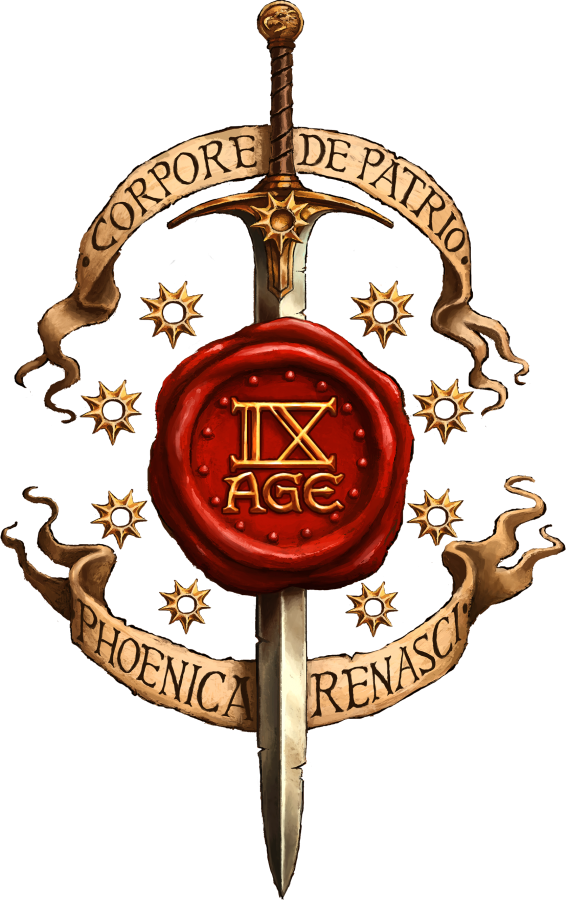
\includegraphics[width=9cm]{../Layout/pics/logo_9th.png}
\vfill
{\antiquefont\fontsize{12}{14.4}\selectfont \textit{\labels@creators}} \\


\end{center}

\newpage

\thispagestyle{empty}

\vphantom{1pt}
\vfill

{\fontsize{12}{14.4}\selectfont

\labels@secondpageannouncement{}

\noindent\newrule{\labels@rulechanges}

\bigskip
\noindent \labels@latexcredit
}


\end{titlepage}

\restoregeometry

\armyspecialrules

\armyspecialruleentry{\masterofundeath}

\newrule{Seule une figurine avec cette règle peut être choisie pour être le Général de l'armée. Le Général est automatiquement le Maître de l'armée et doit échanger l'un de ses sorts par \necromancysignaturespell{}, de la Discipline \necromancy. Au début de n'importe quel tour de joueur pour lequel l'armée n'a plus de Maître en vie, vous devez choisir un personnage utilisant la Discipline \necromancy{} pour le remplacer. S'il passe un test de Commandement avec succès, il devient alors le nouveau Maître de l'armée.}

\armyspecialruleentry{\ashestoashes}

\newrule{À la fin de la phase durant laquelle le Général est retiré en tant que perte,et à chaque fois qu'un test de Commandement est raté pour désigner un nouveau Maître (ou si aucune figurine n'est éligible pour le devenir), chaque unité avec une majorité de figurine possédant cette règle spéciale doit réussir un test de Commandement. Si le test échoue, l'unité subit un nombre de blessures équivalent à la différence entre le résultat obtenu et la valeur de Commandement du test. Ces blessures sont réparties comme pour la règle \unstable{} mais ne peuvent être assignées à une figurine n'ayant pas la règle \ashestoashes{}.}

\armyspecialruleentry{\newrule{\chillingshriek{X, Y}}}

L'élément de figurine avec cette règle spéciale peut effectuer une attaque \newrule{spéciale} de tir de \range{8}. Cette attaque peut être utilisée après une Marche Forcée et touche automatiquement. La cible subit X touches de Force égale à Y plus le nombre de PVs actuels du tireur, X et Y étant les valeurs contenues entre parenthèses. Lorsque vous jetez les dés pour blesser, comparez la Force avec le Commandement de la cible, plutôt que son Endurance. Les blessures infligées ont \armourpiercing{6} et sont des \magicalattacks{}.

Durant la Phase de Corps à Corps, l'élément de figurine peut choisir de remplacer ses attaques normales par un \chillingshriek{} dirigé contre l'une des unités en contact socle à socle avec elle.

\armyspecialruleentry{\awaken{X}}

Une figurine avec cette règle spéciale peut Ressusciter des PVs au-delà de l'effectif de départ de toutes les unités mentionnées entre parenthèses, en suivant les modalités de \raisewounds . L'effectif de départ est le nombre de figurines choisi sur la liste d'armée. Les unités peuvent même dépasser l'effectif maximal autorisé sur leur fiche d'unité.

\armyspecialruleentry{\invocation{X}}

Les figurines et unités avec cette règle spéciale peuvent se faire Ressusciter des PVs par l'\necromancysignaturespell{} (Discipline \necromancy{}) d'un montant de PVs égal à X, contenu entre parenthèses. Une unité ne peut dépasser son effectif d'origine à moins d'être concernée par la règle \awaken{} du lanceur de sort.

\armyspecialruleentry{\reaper}

\newrule{Une unité composée uniquement de figurines suivant cette règle spéciale peut se déplacer au travers d'unités \removedrule{ennemies} durant l'étape des Autres Mouvements. Chaque figurine de l'unité peut alors effectuer une attaque de corps à corps, contre une unité qu'elle a traversée. Ces attaques touchent automatiquement et sont distribuées comme des tirs.}

\armyspecialruleentry{\vampiric{X}}

Une unité \vampiric{} peut effectuer des Marches Forcées même lorsqu'elle se trouve hors de portée de la \inspiringpresence{} du Général. Elle doit toujours effectuer un test de Commandement si elle se trouve dans un rayon de \distance{8} d'une unité ennemie.

\newrule{À la fin de la phase de Combat, les unités avec cette règle spéciale peuvent faire un jet \vampiric{} si une figurine avec cette règle spéciale a causée une blessure non sauvegardée durant cette phase. Lancez 1D6 pour chaque test \vampiric{}, sur un score de X+, un Point de vie est Relevé dans l'unité, où X est le chiffre entre parenthèse (\result{1} est toujours un échec). Les Personnages doivent causer les blessures et lancer le test pour Relever des blessures séparément de l'unité qu'ils ont rejoints.}

\armyspecialruleentry{\wakethedead}

À chaque fois qu'une figurine ayant cette règle spéciale est la cible d'un sort de type Augmentation issu de la Discipline \necromancy (incluant l'attribut \necromancyattribute{}), sélectionnez une unité dans un rayon de \distance{6} de la figurine. Jusqu'à la fin du tour de joueur suivant, toutes les figurines de l'unité sélectionnée ayant la règle \undead{} bénéficient de la règle \lightningreflexes{}.

\armyspecialruleentry{\necromanticaura}

\newrule{Les unités avec cette règle spéciale et les unités à portée d'une ou plusieurs figurines avec cette règle subissent une blessure de moins lorsqu'elles appliquent les règles \unstable{} et \ashestoashes{}. Les unités avec cette règle spéciale ont une portée de \distance{6}. Le Porteur de la Grande Bannière bénéficie automatiquement de cette regle spéciale avec la portée de leur \holdyourground{}.}



\armynewsection{\bloodlines}

Les \vampirelords{} et les \vampireheroes{} peuvent acheter des améliorations uniques appelées \bloodpowers{}, divisées en deux catégories selon leur puissance, les \bloodlinepowers{}, et les \ancientbloodpowers{}. Les Vampires peuvent également être améliorés pour faire partie d'une \bloodline{}, leur donnant des bonus et des restrictions supplémentaires. Les Vampires d'une armée doivent tous faire partie d'une même \bloodline{}, ou alors aucun Vampire ne doit faire partie d'une \bloodline{}. 

\armynewsubsection{Vampires de \bloodline{}}

Ces Vampires ne peuvent acheter que des \bloodpowers{} de leur \bloodline{} . Les \bloodlinepowers{} peuvent être choisis en plusieurs exemplaires, et par n'importe quel Vampire, alors que les \ancientbloodpowers{} sont \oneofakind{} et ne sont accessibles qu'aux \vampirelords{}.

\armynewsubsection{Vampires indépendants}

Un Vampire sans \bloodline{} peut choisir un \bloodlinepowers{} parmi ceux de toutes les \bloodlines{}. Ils sont \oneofakind{}.

\armynewsubsection{\bloodties{X}}
Certaines entrées du livre d'armée sont notées comme étant des \bloodties{}, suivies entre parenthèses de la \bloodline{} à laquelle elles appartiennent. Si vos Vampires font partie de la même \bloodline{} que celle entre parenthèses, vous pouvez alors choisir l'option décrite sur la fiche d'unité.


\separator

\armynewsubsection{\bloodline{} \brotherhood{}\dotfill \pts{35/25}}

Un Vampire \brotherhood{} gagne +2 en Capacité de Combat et porte une \platearmour{}. Il ne peut acheter qu'un seul niveau de magie supplémentaire et ne peut utiliser que la Discipline \necromancy{}. Un Vampire \brotherhood{} ne peut jamais refuser de défi et doit en lancer dès qu'il le peut, à moins qu'un autre Vampire \brotherhood{} ne le fasse en premier.

\bloodties{}: \vampireknights{}.

\startpricelist

\pricelistitem{Rage Écarlate}{65} \textbf{\ancientbloodpower}. Pour chaque blessure non sauvegardée qu'inflige le Vampire au corps à corps, il peut immédiatement effectuer une autre attaque de corps à corps. Ces attaques additionnelles ne génèrent pas d'attaques supplémentaires.

\pricelistitem{\newrule{Maître-Lames}}{35} \textbf{\bloodlinepower}. Le Vampire obtient les règles \weaponmaster{} et \lethalstrike{}. Il est équipé d'une \ahw{}, d'une \halberd{}, d'une \gw{}, d'une \lance{} et d'un \shield{}.

\pricelistitem{\newrule{Avatar de la Mort}}{30} \textbf{\bloodlinepower}. Lorsqu'il combat en défi, le Vampire peut relancer ses jets pour toucher et pour blesser ratés.

\endpricelist

\separator

\armynewsubsection{\bloodline{}  \strigoi{}\dotfill \pts{50/40}}
La figurine du Vampire \strigoi{} gagne +1 Point de Vie, obtient une \regeneration{\newrule{5}} et est sujet à la \hatred{}. Le Vampire ne peut pas sélectionner de monture à l'exception d'une \shriekinghorror{}, ne peut porter aucune Armure, et ne peut acheter qu'un seul niveau de magie supplémentaire. Il doit utiliser les Disciplines \wilderness{} ou \necromancy{}.

\bloodties{}: \ghouls{}.

\startpricelist

\pricelistitem{\newrule{Roi des Goules}}{65} \textbf{\ancientbloodpower}. Le Vampire fait des \poisonedattacks{} et a \armourpiercing{1}. Les Goules de l'unité qu'il rejoint gagnent la \hatred{} et \armourpiercing{1}.

\pricelistitem{Malédiction du Sang}{70} \textbf{\bloodlinepower}. Le Vampire gagne \regeneration{5}. S'il avait déjà la règle \regeneration{}, il améliore de \newrule{1} la sauvegarde qu'elle confère, pour obtenir au mieux 4+. Les Goules dans la même unité que le Vampire et l'éventuelle monture de ce dernier ont la règle spéciale \regeneration{6}, qui augmente d'un point si les figurines possédaient déjà la règle, pour un maximum de 4+.

\pricelistitem{\newrule{Horreur Volante}}{\newrule{65/40}} \textbf{\bloodlinepower}. Figurines à pied uniquement. Le Vampire a \thunderouscharge{} et \fly{8}.

\endpricelist

\separator

\armynewsubsection{\bloodline{} \vonkarnstein{}\dotfill \pts{25/20}}
La présence d'un ou plusieurs Vampires de cette \bloodline{} dans un corps à corps octroie un bonus de +1 au résultat de combat. Une unité avec la règle \undead{} rejointe par un \vonkarnstein{} peut effectuer une Marche Forcée comme si elle était \vampiric{}. La portée de la \inspiringpresence{} et de \holdyourground{} du Vampire est augmentée de \distance{6}, et il peut relancer les jets ratés de \vampiric{}. 

\bloodties{}: \darkcoach .

\startpricelist

\pricelistitem{\newrule{Sombre Tempête}}{50} \textbf{\ancientbloodpower}.  Toutes les unités dans un rayon de \distance{12} autour du Vampire ont la règle spéciale \blurry . De plus, une fois par partie, le Vampire peut avoir, ainsi que toute unité qu'il aurait rejointe, les règles spéciales \lightningattacks{} et \armourpiercing{2}. Cette capacité doit être activée au début d'une Phase de Corps à Corps et dure jusqu'à la fin du tour de joueur.

\pricelistitem{Goût Raffiné}{25} \textbf{\bloodlinepower}. Le Vampire obtient \vampiric{2}, ou \vampiric{4} s'il est monté sur une \largetarget{}.

\pricelistitem{Maître de la Nuit}{20} \textbf{\bloodlinepower}. Le Vampire gagne \awaken{\zombies, \direwolves, \batswarms, \greatbats}, et le Vampire ainsi que l'unité qu'il rejoint gagnent la règle \swiftstride{}.

\endpricelist

\separator

\armynewsubsection{\lamia{} \bloodline\dotfill \pts{35/25}}
La Vampire gagne +2 en Capacité de Tir, perd une Attaque, et obtient la règle \lightningreflexes{} et des \throwingweapons{}. Si elle ne porte aucune Armure, elle obtient également la règle \distracting{}.

\bloodties{}: \courtofthedamned .

\startpricelist

\pricelistitem{Commandement}{50} \textbf{\ancientbloodpower}. Toute les figurines ordinaires de l'unité rejointe par la Vampire obtiennent une Capacité de Combat de 5. Si la Vampire n'est pas engagée au corps à corps, elle peut à la place choisir de donner ce bonus à une unique unité située dans un rayon de \distance{6}.

\pricelistitem{\newrule{Danse Enchanteresse}}{25} \textbf{\bloodlinepower}. Les unités au contact d'un ou plusieurs Vampires avec ce pouvoir ont -1 en Commandement.

\pricelistitem{\newrule{Regard Hypnotique}}{25} \textbf{\bloodlinepower}. Une unité chargeant ou fuyant face à une unité avec un ou plusieurs Vampires ayant ce pouvoir lance un dé supplémentaire pour son mouvement de charge ou fuite et retire le dé avec le plus haut résultat.

\endpricelist

\separator

\armynewsubsection{\bloodline{} \nosferatu{}\dotfill \pts{\newrule{140/70}}}
Le Vampire est un \wizard{} de niveau 4/2, il a -1 Attaque et -2 en Capacité de Combat, et ne peut porter aucune armure. Il génère un sort supplémentaire et a la règle spéciale \awaken{\zombies, \skeletons}. Un Vampire \nosferatu{} peut générer ses sorts dans plusieurs Disciplines magiques. Les Disciplines choisies et combien de sorts sont générés dans chaque Discipline doivent figurer dans la liste d'armée.

\bloodties{}: \wraiths .

\startpricelist

\pricelistitem{\newrule{Maîtrise des Arts Noirs}}{50} \textbf{\ancientbloodpower}. Au début de chaque Phase de Magie, le joueur peut désigner un \wizard ennemi, situé en ligne de vue et dans un rayon de \distance{18} du Vampire. Ce Sorcier ne peut ajouter son niveau de magie ou utiliser la règle \aideddispel{} contre les sorts lancés par le Vampire durant cette phase. 

\pricelistitem{Sang Royal}{25} \textbf{\bloodlinepower}. Les sorts lancés par le Vampire et n'étant pas de type Vortex voient leur Portée augmentée de \distance{6} pour les sorts de Dommages, et de \distance{3} pour les autres types de sorts.

\pricelistitem{Voies Interdites}{20} \textbf{\bloodlinepower}. Sélectionnez une Discipline \battle{} autre que celle \nature{}. Le Vampire peut également choisir cette Discipline pour générer ses sorts en plus de celles normalement accessibles.

\endpricelist

\armymagicitems

\armymagicweapons

\startpricelist

\pricelistitem{\newrule{L'Arc Ancien}}{45} Type : \artilleryweapon{}, \boltthrower{}. \range{36}, Force 6, \armourpiercing{1}, \multiplewounds{1D3}{}.

\pricelistitem{Lame de la Soif Rouge}{40} \newrule{\only{Vampires}}. Type: \hw . \newrule{Le Vampire maniant cette lame gagne \vampiric{5} s'il est monté sur une \largetarget{}, sinon il gagne \vampiric{3}. L'élément de la figurine lance 1D6 pour \newrule{chaque} blessure qu'il inflige dans le cadre de sa regle \vampiric{}. Tout excès de blessures ainsi soignées peut être utilisé pour \raisewounds{} dans l'unité que le personnage a rejointe.}

\endpricelist

\armymagicarmor

\startpricelist

\pricelistitem{Haubert Sanglant}{\newrule{40}} Type : \platearmour{}. Le porteur gagne +1 Point de Vie.

\endpricelist

\armytalismans

\startpricelist

\pricelistitem{\newrule{Linceul de Nuit}}{40} Figurine à pied uniquement. Les figurines au contact du porteur ainsi que toute figurine allouant ses attaques sur le porteur ne reçoivent aucun bonus de \newrule{type +X en} Force lié à leurs armes, qu'elles soient magiques ou ordinaires.

\endpricelist

\armyenchanteditems

\startpricelist

\pricelistitem{\newrule{Livre Maudit}}{\newrule{50}} \removedrule{Figurine à pied uniquement}. Le porteur et toute figurine ordinaire de son unité gagnent la règle \distracting{}.

\endpricelist

\armyarcaneitems

\startpricelist

\pricelistitem{Tome Impie}{35} \boundspell{4}. Cet objet permet de lancer \necromancyspelltwo{} (Discipline \necromancy{}).

\pricelistitem{Baguette d'Asservissement}{35} \boundspell{3}. Amélioration, \range{6}, Dure un tour. Toutes les figurines de l'unité ciblée gagnent +1 Attaque.

\pricelistitem{Charme des Ténèbres}{20} À la fin de n'importe quelle Phase de Magie, vous pouvez mettre un dé de magie inutilisé de côté pour l'ajouter à votre réserve du tour suivant, juste après avoir déterminé les vents de magie.

\endpricelist

\armymagicbanners

\startpricelist

\pricelistitem{Armoiries de Castelhof}{75} L'unité gagne \bodyguard{\vampirelord, \vampirehero}. Les \vampireknights{} portant cette bannière gagnent à la place la règle \stubborn{}. Toutes les figurines de l'unité obtiennent de surcroît une \wardsave{4} contre toute attaque à distance. 

\pricelistitem{Bannière des Tertres}{50} Les figurines de \barrowknights, \barrowguards{} et \barrowkings{} de l'unité obtiennent +1 pour toucher au corps à corps.

\endpricelist




%%%%%%%%%%%%%%%%%%%%%%%%%%%%%%%%%%%%%%%%%%%%%%%%%%%%%%%%%%%%%%%%%%%%%%%%%%%%%%%%%%%%%%%%%%%%%%%%%
%%%%%																						%%%%%
%%%%% TRANSLATORS SHOULDN'T HAVE TO EDIT THE CODE PAST THIS LINE - TRANSLATION IS AUTOMATED %%%%%
%%%%%					(unless you want to edit the changelog)								%%%%%
%%%%%%%%%%%%%%%%%%%%%%%%%%%%%%%%%%%%%%%%%%%%%%%%%%%%%%%%%%%%%%%%%%%%%%%%%%%%%%%%%%%%%%%%%%%%%%%%%



\armylist

\lordstitle

\showunit{
	name={\vampirelord},
	cost={200},
	profile={ < 6 7 5 5 5 3 7 5 10},
	type=\infantry ,
	basesize=20x20,
	unitsize=1,
	commontype=\vampiriccommonrules ,
	commonspecialrules={\undead,\fear,\vampiric{6}},
	specialrules={\awaken{\zombies},\masterofundeath},
	magiclevel=1,
	magicpaths={\necromancy, \shadows, \death},
	options={
		\bloodlinechoice = \unlimited,
		\bloodpowerchoice = \unlimited,
		\magicitemsallowance = \upto < 100,
		\magiclevelchoice{
			\magiclevel{2}=30,
			\magiclevel{3}=75,
		},
		\anyofthefollowing{
			\la =5,
			\ha =10,
			\shield =5,
		},
		\weapononechoice{
			\ahw =5,
			\halberd =10,
			\gw =15,
			\lance =\newrule{20},
		}
	},
	mounts={\skeletalsteed =20, \monstrousrevenant =100, \courtofthedamned{} \only{\lamia}=190, \shriekinghorror{} \only{\strigoi}=200, \zombiedragon =280}
}

\showunit{
	name={\necromancerlord},
	cost={150},
	profile={ < 4 3 3 3 4 3 3 1 8},
	type= \infantry ,
	basesize=20x20,
	unitsize=1,
	commontype=\undeadcommonrules ,
	commonspecialrules={\undead},
	specialrules={\awaken{\zombies , \skeletons}, \masterofundeath},
	magiclevel=3,
	magicpaths={\necromancy, \fire, \death},
	options={
		\magicitemsallowance = \upto < 100,
		\magiclevel{4}=60,
	},
	mounts={\skeletalsteed =20, \monstrousrevenant =100, \cadaverwagon =100}
}

\heroestitle


\showunit {
	name={\vampirehero},
	cost=80,
	profile={ < 6 6 4 5 4 2 6 4 8},
	type=\infantry ,
	basesize=20x20,
	unitsize=1,
	commontype=\vampiriccommonrules ,
	commonspecialrules={\undead,\fear,\vampiric{6}},
	specialrules={\awaken{\zombies}, \masterofundeath},
	magicpaths={\necromancy, \shadows, \death},
	options={
		\bloodlinechoice =\unlimited,
		\bloodpowerchoice =\unlimited,		
		\magicitemsallowance = \upto < 50,
		\bsboption{} \notif{\strigoi}= 25,
		\magiclevelchoice{
			\magiclevel{1}=25,
			\magiclevel{2}=55,
		},
		\anyofthefollowing{
			\la =5,
			\ha =10,
			\shield =5,
		},
		\weapononechoice{
			\ahw =5,
			\halberd =5,
			\gw =10,
			\lance =\newrule{15},
		}
	},
	mounts={\skeletalsteed =20, \monstrousrevenant =120}
}


\showunit{
	name={\necromancer},
	cost={60},
	profile={ < 4 3 3 3 3 2 3 1 7},
	type= \infantry ,
	basesize=20x20,
	unitsize=1,
	commontype=\undeadcommonrules ,
	commonspecialrules={\undead},
	specialrules={\awaken{\zombies, \skeletons}, \masterofundeath},
	magiclevel=1,
	magicpaths={\necromancy, \fire, \death},
	options={
		\magicitemsallowance = \upto < 50,
		\magiclevel{2}=30,
	},
	mounts={\skeletalsteed = \newrule{20}, \cadaverwagon = 100}
}

\showunit{
	name={\barrowking},
	cost=80,
	profile={ < 4 4 - 4 5 3 4 3 9},
	type=\infantry ,
	basesize=20x20,
	unitsize=1,
	commontype=\undeadcommonrules ,
	commonspecialrules={\undead},
	specialrules={\multiplewounds{2}{\infantry, \cavalry, \warbeasts}, \lethalstrike, \notaleader, \newrule{\magicalattacks}},
	equipment={\ha, \shield},
	options={
		\magicitemsallowance = \upto < 50,
		\bsboption = 25,
		\weapononechoice{
			\ahw =5,
			\halberd =5,
			\lance =5,
			\gw =10,
		},
		\maybeupgradedto{} \unlivingshield = 15
	},
	mounts={\skeletalsteed = \newrule{20}},
	unitrules={
		\unitrule{\unlivingshield}{\unlivingshieldrule}
	}
}

\showunit {
	name={\fellwraith},
	cost=65,
	profile={\fellwraith < 6 3 - 3 3 2 2 \newrule{3} 5,
		     \banshee 	 < 6 3 - 3 3 2 3 \newrule{1} 5
	},
	type=\infantry ,
	basesize=20x20,
	unitsize=1,
	commontype=\undeadcommonrules ,
	commonspecialrules={\undead, \ashestoashes},
	specialrules={\ethereal, \reaper, \notaleader, \terror},
	options={
		\mustbecomeoneofthefollowing{
			\fellwraith = \free,
			\banshee = 30
		}
	},
	additional={%
		\separator
		\begin{multicols}{2}
		\begin{center} \LARGE\antiquefont\fellwraith \end{center}
		
		{\setlength{\parskip}{0.1cm}
			\noindent\textbf{\labels@specialrules :}\expandafter\ruleslist\expandafter{%
				\armourpiercing{6}%
			}.
		
			\noindent\textbf{\labels@equipment :}\expandafter\equipmentlist\expandafter{%
				\gw%
			}.
		}

		\vspace*{0.15cm}\mountsframestart\expandafter\mountslist\expandafter{%
			\newrule{\skeletalsteed} = \newrule{20}%
		}\mountsframeend
			
		\columnbreak
		\begin{center} \LARGE\antiquefont\banshee \end{center}
		
		\noindent\textbf{\labels@specialrules :}\expandafter\ruleslist\expandafter{%
			\chillingshriek{2, 8}%
		}.
		\end{multicols}
	},
}


\coreunitstitle

\showunit{
	name={\zombies},
	cost=60,
	profile={ < 4 1 0 3 3 1 1 1 2},
	invocation={2D6+3},
	type=\infantry ,
	basesize=20x20,
	unitsize=20,
	additionalmodels=40,
	costpermodel=3,
	commontype=\undeadcommonrules ,
	commonspecialrules={\undead, \ashestoashes},
	commandgroup={musician=10, banner=10}
}

\showunit{
	name={\skeletons},
	cost=40,
	profile={< 4 2 2 3 3 1 2 1 6},
	invocation={1D6+3},
	type=\infantry ,
	basesize=20x20,
	unitsize=10,
	additionalmodels=50,
	costpermodel=4,
	commontype=\undeadcommonrules ,
	commonspecialrules={\undead, \ashestoashes},
	equipment={\la},
	options={
		\spear = \free,
		\shield = \permodel < 1
	},
	commandgroup={champion=10, musician=10, banner=10, veteranbannerallowance=\newrule{25}}
}

\showunit{
	name={\ghouls},
	cost=90,
	profile={< 4 3 - 3 4 1 3 2 6},
	invocation={1D6+3},
	type= \infantry ,
	basesize=20x20,
	unitsize=10,
	additionalmodels=30,
	costpermodel=9,
	commontype=\undeadcommonrules ,
	commonspecialrules={\undead, \ashestoashes},
	specialrules={\poisonedattacks},
	options={
		\skirmishers{} \ifNmodelsorless{15}= \permodel < 1,
		\bloodties{\strigoi}:\newline\vanguard{}*= \permodel < 2,
	},
	commandgroup={champion=10, musician=10, bannerrestriction=\unitwith{} \vanguard , banner=10, musicianrestriction=\unitwith{} \vanguard , veteranbannerallowance = \newrule{25}},
	additional={%
		\vspace*{0.1cm}		
		* \strigoivanguardnote
	}
}

\showunit{
	name={\direwolves},
	cost=40,
	profile={
		< 9 3 0 3 3 1 3 1 3},
	invocation={1D3+3},
	type=\warbeast ,
	basesize=25x50,
	unitsize=5,
	additionalmodels=10,
	costpermodel=7,
	commontype=\undeadcommonrules ,
	commonspecialrules={\undead, \ashestoashes},
	specialrules={\vanguard, \thunderouscharge},
	commandgroup={champion=10}
}

\showunit{
	name={\batswarm},
	cost=60,
	profile={
		< 1 2 - 2 2 4 3 4 3},
	invocation={1D6+3},
	type=\swarm ,
	basesize=40x40,
	unitsize=2,
	additionalmodels=8,
	costpermodel=15,
	commontype=\undeadcommonrules ,
	commonspecialrules={\undead, \ashestoashes},
	specialrules={\fly{6}},
	unitrules={
		\unitrule{\stormofwings}{\stormofwingsrule}
	}
}

\specialunitstitle


\showunit{
	name={\barrowknights},
	cost=120,
	profile={\knight < 4 3 - 4 4 1 3 1 6,
			  \steed < 8 2 - 3 3 1 2 1 3
	},
	invocation= 2 ,
	type=\cavalry ,
	basesize=25x50,
	unitsize=5,
	additionalmodels=10,
	costpermodel=24,
	commontype=\undeadcommonrules ,
	commonspecialrules={\undead, \ashestoashes},
	specialrules={\magicalattacks, \multiplewounds{2}{\infantry , \cavalry , \warbeasts}, \lethalstrike{} \only{\knight}, \ethereal{} \only{\steed}},
	equipment={\ha , \shield , \lance , \mountsprotection{5}},
	commandgroup={champion=10, musician=10, banner=10, bannerallowance=50}
}

\showunit{
	name={\barrowguards},
	cost=100,
	profile={
		< 4 3 - 4 4 1 3 1 8},
	invocation= 1D3+3 ,
	type=\infantry,
	basesize=20x20,
	unitsize=10,
	additionalmodels=30,
	costpermodel=10,
	commontype=\undeadcommonrules ,
	commonspecialrules={\undead, \ashestoashes},
	specialrules={\magicalattacks, \multiplewounds{2}{\infantry , \cavalry , \warbeasts},\lethalstrike, \bodyguard{\general, \barrowking}},
	equipment={\ha},
	options={
		\shield = \permodel < 1,
		\weapononechoice{
			\halberd = \permodel < 2,
			\gw = \permodel < 2
		},
	},
	commandgroup={champion=10, musician=10, banner=10, bannerallowance=50}
}

\showunit{
	name={\ghasts},
	cost=110,
	profile={< 6 3 - 4 5 3 2 3 5},
	invocation= 2 ,
	type=\monstrousinfantry ,
	basesize=40x40,
	unitsize=3,
	additionalmodels=7,
	costpermodel=48,
	commontype=\undeadcommonrules ,
	commonspecialrules={\undead, \ashestoashes},
	specialrules={\poisonedattacks, \fear,  \regeneration{5}},
	commandgroup={champion=10}
}

\showunit{
	name={\vampirespawn},
	cost=126,
	profile={
		< 6 4 - 5 4 3 4 3 8},
	invocation= 2 ,
	type=\monstrousinfantry ,
	basesize=40x40,
	unitsize=3,
	additionalmodels=5,
	costpermodel=42,
	commontype=\vampiriccommonrules ,
	commonspecialrules={\undead, \vampiric{6}, \fear},
	specialrules={\frenzy, \skirmishers, \fly{9}},
	commandgroup={champion=10}
}

\showunit{
	name={\phantomhost},
	cost=70,
	profile={< 6 3 - 3 3 4 1 4 4},
	invocation= 1D3+3 ,
	type=\infantry,
	basesize=40x40,
	unitsize=2,
	additionalmodels=4,
	costpermodel=35,
	commontype=\undeadcommonrules ,
	commonspecialrules={\undead, \ashestoashes},
	specialrules={\ethereal, \fear}
}

\showunit{
	name={\greatbats},
	cost=40,
	profile={
		< 1 3 - 3 3 2 3 2 3},
	invocation= 1D3+3 ,
	type=\warbeast ,
	basesize=40x40,
	unitsize=2,
	additionalmodels=7,
	costpermodel=14,
	commontype=\undeadcommonrules ,
	commonspecialrules={\undead, \ashestoashes},
	specialrules={\skirmishers, \fly{10}},
}

\showunit{
	name={\varkolak},
	cost=\newrule{165},
	profile={
		< 8 5 - 6 5 4 4 5 7},
	invocation= 1 ,
	type=\monstrousbeast ,
	basesize=50x50,
	unitsize=1,
	commontype=\vampiriccommonrules ,
	commonspecialrules={\undead, \vampiric{3}, \fear},
	specialrules={\hatred, \regeneration{4}},
	options={
		\maytakeoneofthefollowing{
			\vanguard{}= 20,
			\stomp{1D3+1}= 20,
			\fly{8}= 40,
		}
	}
}

\showunit{
	name={\cadaverwagon},
	cost=80,
	profile={
		\cadaverwagon < - - - 4 4 4 - - -,
   		\cadavermaster < - 3 - 3 - -  3 1 5,
		\shamblinghorde < 4 1 - 3 3 -  1 * -	
	},
	invocation= 1 ,
	type=\chariot ,
	basesize=50x100,
	unitsize=1,
	commontype=\undeadcommonrules ,
	commonspecialrules={\undead, \ashestoashes},
	specialrules={\randomattacks{2D6} \only{\shamblinghorde}, \wakethedead, \cart, \regeneration{4}},
	equipment={\mountsprotection{5}},
	options={
		\endlesshorde = 25,
		\maytakeoneofthefollowing{
			\bonepyre = 10,
			\bringoutyourdead = 15,
			\necromanticaura = 20
		}
	},
	unitrules={
		\unitrule{\cart}{\cartrule}
		\unitrule{\endlesshorde}{\endlesshorderule}
		\unitrule{\bonepyre}{\bonepyrerule}
		\unitrule{\bringoutyourdead}{\bringoutyourdeadrule}
	}
}

\rareunitstitle


\showunit{
	name={\vampireknights},
	cost=225,
	profile={
		\knight < 4 5 3 5 4 2 5 2 8,
		\undeadmount < 8 3 0 4 3 1 2 1 3
	},
	invocation= 2 ,
	type=\cavalry ,
	basesize=25x50,
	unitsize=5,
	additionalmodels=5,
	costpermodel=45,
	commontype=\vampiriccommonrules ,
	commonspecialrules={\undead,\fear,\vampiric{6}},
	equipment={\lance , \ha , \shield , \mountsprotection{6}, \barding},
	options={
		\bloodties{\brotherhood}:\newline\platearmour{} \wordand{} \devastatingcharge{}= \permodel < 15
	},
	commandgroup={champion=10, musician=10, banner=10, bannerallowance=75}
}

\showunit{
	name={\wraiths},
	cost=\newrule{150},
	profile={
		< 6 3 - 3 3 2 2 2 5
	},
	invocation= 2,
	type=\infantry,
	basesize=20x20,
	unitsize=5,
	additionalmodels=\newrule{3},
	costpermodel=\newrule{30},
	commontype=\undeadcommonrules ,
	commonspecialrules={\undead, \ashestoashes},
	specialrules={\wizardconclave{\Level{} \newrule{2}, \deathsignaturespell{} (Path of \death), \newrule{\shadowssignaturespell{} (Path of \shadows)}}, \ethereal,  \bodyguard{\fellwraith , \banshee}, \reaper, \armourpiercing{6}, \terror, \skirmishers},
	equipment={\gw},
	commandgroup={champion=70, championprerestriction=\bloodties{\nosferatu}:},
}

\showunit{
	name={\mountedwraiths},
	cost=150,
	profile={\rider < 6 3 - 3 3 1 2 1 5,
	         \steed < 8 2 - 3 3 1 2 1 3
	},
	invocation= 2,
	type=\cavalry ,
	basesize=25x50,
	unitsize=5,
	additionalmodels=5,
	costpermodel=30,
	commontype=\undeadcommonrules ,
	commonspecialrules={\undead, \ashestoashes},
	specialrules={\flamingattacks{} \only{\rider}, \ethereal, \reaper, \armourpiercing{6} \only{\rider}, \freereform, \terror},
	equipment={\gw , \mountsprotection{6}},
	commandgroup={champion=10}
}

\showunit{
	name={\wingedreapers},
	cost=150,
	profile={
        	< 6 5 3 5 5 4 4 3 10,
	},
	invocation= 2,
	type=\monstrousinfantry ,
	basesize=50x75,
	unitsize=2,
	additionalmodels=3,
	costpermodel=75,
	commontype=\undeadcommonrules ,
	commonspecialrules={\undead, \ashestoashes},
	specialrules={\necromanticaura, \undeadconstructs, \lethalstrike, \terror, \fly{6}},
	equipment={\innatedefence{5}},
	options={
			\la = \permodel < 10,
		\weapononechoice{
			\ahw = \permodel < 5,
			\halberd = \permodel < 10
		}
	},
	unitrules={
		\unitrule{\undeadconstructs}{\undeadconstructsrule}
	},
}

\showunit{
	name={\altarofundeath},
	cost=200,
	profile={
		\altarofundeath < -  - - 5 5 5 - - -,
       	\master{} (1) < -  3 1 3 - - 3 1 5,
		\banshee{} (0)[1] < -  3 - 3 - [2] 3 3 5,
		\ghoststeeds{} (1) < 8 3 - 3 - - 2 * 4
	},
	invocation= 1,
	type=\chariot ,
	basesize=50x100,
	unitsize=1,
	commontype=\undeadcommonrules ,
	commonspecialrules={\undead, \ashestoashes},
	specialrules={\randomattacks{2D6} \only{\ghoststeeds}, \auraofundeath, \chillingshriek{2,8} \only{\banshee},  \ethereal{} \only{\ghoststeeds}, \largetarget , \terror , \regeneration{4}},
	equipment={\innatedefence{5}},
	options={
		\maytakeoneofthefollowing{
			\banshee{} (1)= 20,
			\darktome = 20
		}
	},
	unitrules={
		\unitrule{\darktome}{\darktomerule}
		\unitrule{\auraofundeath}{\auraofundeathrule}
	}
}

\showunit{
	name={\shriekinghorror},
	cost=200,
	profile={
        	< 6 4 - 5 6 6 2 4 4,
	},
	invocation= 1,
	type=\monster ,
	basesize=100x150,
	unitsize=1,
	commontype=\undeadcommonrules ,
	commonspecialrules={\undead, \ashestoashes},
	specialrules={\chillingshriek{6, 4}, \regeneration{6}, \fly{8}},
}

\showunit{
	name={\darkcoach},
	cost=190,
	profile={
		\darkcoach 				< - - - 5 6 4 - - -,
        \fellwraith{} (1) 		< - 3 - 3 - - 3 3 5,
		\awakenedvampire{} (*) 	< - 6 - 5 - - 6 4 8,
		\undeadmount{} (2) 		< 8 3 - 4 - - 2 1 -
	},
	invocation= 1,
	type=\chariot ,
	basesize=50x100,
	unitsize=1,
	commontype=\vampiriccommonrules ,
	commonspecialrules={\undead , \vampiric{4}},
	specialrules={\soulsyphon, \scythes, \wardsave{4}, \terror},
	equipment={\ha, \mountsprotection{5}, \gw{} \only{\fellwraith}},
	options={
		\bloodties{\vonkarnstein}:\newline\stubborn = 30
	},
	unitrules={
		\unitrule{\soulsyphon}{\soulsyphonrule}
	},
	additional={\soulsyphonchart},
}

\showunit{
	name={\courtofthedamned},
	cost=190,
	profile={
		\courtofthedamned 	< - - - 5 5 5 - - -,
       	\paramours{} (3) 	< - 5 5 5 - - 6 2 7,
		\ghoststeeds{} (1) 	< 8 3 - 3 - - 2 * 4
	},
	invocation= 1,
	type=\chariot ,
	basesize=50x100,
	unitsize=1,
	commontype=\vampiriccommonrules ,
	commonspecialrules={\undead , \vampiric{6}},
	specialrules={\randomattacks{2D6} \only{\ghoststeeds}, \ethereal{} \only{\ghoststeeds}, \largetarget, \wardsave{4}, \terror},
	equipment={\throwingweapons{} \only{\paramours}, \innatedefence{5}},
	options={
		\bloodties{\lamia}:\newline\wakethedead = 25
	}
}


\mountstitle

\mountssectionannouncement

\showunit{
	name={\skeletalsteed},
	cost={-},
	profile={
        		 < 8 2 - 3 3 1 2 1 3,
	},
	type=\warbeast ,
	basesize=25x50,
	unitsize=1,
	commontype=\undeadcommonrules ,
	commonspecialrules={\undead},
	specialrules={\ethereal{} \only{\steed}},
	equipment={\mountsprotection{6}},
	options={
		\maytakeoneofthefollowing{
			\mountsprotection{5}= \newrule{15},
			\fly{8} \newrule{\onlyasvampiresmount}= \newrule{35}
		}
	}
}

\showunit{
	name={\monstrousrevenant},
	cost={-},
	profile={
		< 6  4 - 5 5 4 2 4 4,
	},
	type=\monstrousbeast ,
	basesize=50x50,
	unitsize=1,
	commontype=\undeadcommonrules ,
	commonspecialrules={\undead},
	specialrules={\largetarget, \fear},
	options={%
		\maytakeuptotwoofthefollowing{
			\poisonedattacks = 5,
			\lethalstrike = 10,
			\vampiric{5}= 15,
			\randomattacks{D6+2}= 30,
			\fly{8}= 40
		},
	}
}


\showunit{
	name={\shriekinghorror},
	cost={-},
	profile={
        	< 6 4 - 5 6 6 2 4 4,
	},
	type=Monstre,
	basesize=100x150,
	unitsize=1,
	commontype=\undeadcommonrules ,
	commonspecialrules={\undead},
	specialrules={\chillingshriek{6,4}, \regeneration{6}, \fly{8}},
}

\showunit{
	name={\cadaverwagon},
	cost=80,
	profile={
		\cadaverwagon < - - - 4 4 4 - - -,
		\shamblinghorde < 4 1 - 3 3 -  1 * -	
	},
	type=\chariot ,
	basesize=50x100,
	unitsize=1,
	commontype=\undeadcommonrules ,
	commonspecialrules={\undead},
	specialrules={\randomattacks{2D6} \only{\shamblinghorde}, \wakethedead, \cart, \regeneration{4}},
	equipment={\mountsprotection{5}},
	options={
		\endlesshorde = 25,
		\maytakeoneofthefollowing{
			\bonepyre = 10,
			\bringoutyourdead = 15,
			\necromanticaura = 20
		}
	},
	unitrules={
		\unitrule{\cart}{\cartrule}
		\unitrule{\endlesshorde}{\endlesshorderule}
		\unitrule{\bonepyre}{\bonepyrerule}
		\unitrule{\bringoutyourdead}{\bringoutyourdeadrule}
	}
}

\showunit{
	name={\courtofthedamned},
	cost=190,
	profile={
		\courtofthedamned 	< - - - 5 5 5 - - -,
       	\paramours{} (2) 	< - 5 5 5 - - 6 2 7,
		\ghoststeeds{} (1) 	< 8 3 - 3 - - 2 * 4
	},
	type=\chariot ,
	basesize=50x100,
	unitsize=1,
	commontype=\vampiriccommonrules ,
	commonspecialrules={\undead , \vampiric{6}},
	specialrules={\randomattacks{2D6} \only{\ghoststeeds}, \ethereal{} \only{\ghoststeeds}, \largetarget, \wardsave{4}, \terror},
	equipment={\throwingweapons{} \only{\paramours}, \innatedefence{5}},
	options={
		\bloodties{\lamia}:\newline\wakethedead = 25
	}
}

\showunit{
	name={\zombiedragon},
	cost={-},
	profile={
		< 6  4 - 6 6 6 2 5 4,
	},
	type=\monster ,
	basesize=50x100,
	unitsize={1},
	commontype=\undeadcommonrules ,
	commonspecialrules={\undead},
	specialrules={\breathweapon{\Strength{} 2, \armourpiercing{6}}, \distracting, \regeneration{6}, \fly{7}},
	equipment={\innatedefence{4}},
	options={
		\maybeupgradedto{} \colossalzombiedragon{}= 40
	},
	unitrules={
		\unitrule{\colossalzombiedragon}{\colossalzombiedragonrule}
	}
}

\quickrefsheettitle

% Script to automatically draw the Quick Ref Sheet

\renewcommand{\arraystretch}{1.2}

\providebool{QRSbool}

\providebool{whiterow}

\newcommand{\QRSrowcolor}{\ifbool{whiterow}{\global\boolfalse{whiterow}}{\rowcolor{black!10}\global\booltrue{whiterow}}}

\newcommand{\QRSstarttab}[1]{%
	\noindent%
	\setlength{\tabcolsep}{2pt}%
	\begin{tabular}{@{}cp{3.2cm}M{\profilecellsize}@{}M{\profilecellsize}@{}M{\profilecellsize}@{}M{\profilecellsize}@{}M{\profilecellsize}@{}M{\profilecellsize}@{}M{\profilecellsize}@{}M{\profilecellsize}@{}M{\profilecellsize}}%

	& \antiquefont\large{\textbf{#1}} & \textbf{\labels@M} & \textbf{\labels@WS} & \textbf{\labels@BS} & \textbf{\labels@S} & \textbf{\labels@T} & \textbf{\labels@W} & \textbf{\labels@I} & \textbf{\labels@A} & \textbf{\labels@Ld}%
}%

\newcommand{\QRSclosetab}{\end{tabular}\bigskip}%

\newcommand{\QRSprintline}[4]{%
	\tabularnewline%
	\ifnumequal{\rowmulti}{1}{\QRSrowcolor}{}%
	\DTLifeq*{\rowcategory}{\labels@lords}{\antiquefont\bfseries \labels@lordsInitial}{}%
	\DTLifeq*{\rowcategory}{\labels@heroes}{\antiquefont\bfseries \labels@heroesInitial}{}%
	\DTLifeq*{\rowcategory}{\labels@coreunits}{\antiquefont\bfseries \labels@coreunitsInitial}{}%
	\DTLifeq*{\rowcategory}{\labels@specialunits}{\antiquefont\bfseries \labels@specialunitsInitial}{}%
	\DTLifeq*{\rowcategory}{\labels@rareunits}{\antiquefont\bfseries \labels@rareunitsInitial}{}%
	\DTLifeq*{\rowcategory}{\labels@mounts}{\antiquefont\bfseries \labels@mountsInitial}{}%
	&%
	\ifnumequal{\rowmulti}{1}{%no Multiprofile
		\rowname%
		\expandafter\parselist\expandafter{\rowprofile}{\locallists@profileslist}%
		\forlistloop{\QRSmonoprofile}{\locallists@profileslist}%
	}{% Multiprofile
		\rowname &&&&&&&&&%
		\expandafter\parselist\expandafter{\rowprofile}{\locallists@profileslist}%
		\forlistloop{\QRSmultiprofile}{\locallists@profileslist}%
	}%
}

\newcommand{\QRSmultiprofile}[1]{%
	\tabularnewline%
	\QRSrowcolor{}&%
	\splitatinf{#1}\local@unitname\local@unitprofile%
	- \local@unitname \expandafter\caraclist\expandafter{\local@unitprofile}%
}%

\newcommand{\QRSmonoprofile}[1]{%
	\splitatinf{#1}\local@unitname\local@unitprofile%
	\expandafter\caraclist\expandafter{\local@unitprofile}%
}%

\newcommand{\QRSprinttab}[1]{%
	\global\booltrue{whiterow}%
	\DTLforeach*[#1]%
	{profiles}{\rowname=name, \rowtrooptype=trooptype, \rowcategory=category, \rowprofile=profile, \rowmulti=multipleprofile}{%
      		\QRSprintline{\rowname}{\rowcategory}{\rowprofile}{\rowmulti}%
	}%
}%

\providebool{QRSisempty}
\global\boolfalse{QRSisempty}%

\newcommand{\QRScheckifempty}[1]{%
	\global\booltrue{QRSisempty}%
	\DTLforeach*[#1]%
	{profiles}{\rowname=name, \rowtrooptype=trooptype, \rowcategory=category, \rowprofile=profile, \rowmulti=multipleprofile}{%
		\global\boolfalse{QRSisempty}\dtlbreak%
	}%
}%

\newcommand{\QRSifnotempty}[1]{%
	\ifbool{QRSisempty}{}{#1}%
}%

\begin{multicols}{2}

\QRScheckifempty{%
	\DTLiseq{\rowcategory}{\labels@lords}\or\DTLiseq{\rowcategory}{\labels@heroes}%
}%
\QRSifnotempty{%
	\QRSstarttab{\characters}%
	\QRSprinttab{%
		\DTLiseq{\rowcategory}{\labels@lords}\or\DTLiseq{\rowcategory}{\labels@heroes}%
	}%
	\QRSclosetab{}%
}%

\QRScheckifempty{%
	\DTLiseq{\rowtrooptype}{\infantry}\and\not\DTLiseq{\rowcategory}{\labels@heroes}\and\not\DTLiseq{\rowcategory}{\labels@lords}%
}%
\QRSifnotempty{%
	\QRSstarttab{\infantry}%
	\QRSprinttab{%
		\DTLiseq{\rowtrooptype}{\infantry}\and\not\DTLiseq{\rowcategory}{\labels@heroes}\and\not\DTLiseq{\rowcategory}{\labels@lords}%
	}% 
	\QRSclosetab{}%
}% 

\QRScheckifempty{%
	\DTLiseq{\rowtrooptype}{\monstrousinfantry}\and\not\DTLiseq{\rowcategory}{\labels@heroes}\and\not\DTLiseq{\rowcategory}{\labels@lords}%
}%
\QRSifnotempty{%
	\QRSstarttab{\monstrousinfantry}%
	\QRSprinttab{%
		\DTLiseq{\rowtrooptype}{\monstrousinfantry}\and\not\DTLiseq{\rowcategory}{\labels@heroes}\and\not\DTLiseq{\rowcategory}{\labels@lords}%
	}% 
	\QRSclosetab{}%
}% 

\QRScheckifempty{%
	\DTLiseq{\rowtrooptype}{\warbeast}\and\not\DTLiseq{\rowcategory}{\labels@heroes}\and\not\DTLiseq{\rowcategory}{\labels@lords}%
}%
\QRSifnotempty{%
	\QRSstarttab{\warbeasts}%
	\QRSprinttab{%
		\DTLiseq{\rowtrooptype}{\warbeast}\and\not\DTLiseq{\rowcategory}{\labels@heroes}\and\not\DTLiseq{\rowcategory}{\labels@lords}%
	}% 
	\QRSclosetab{}%
}% 

\QRScheckifempty{%
	\DTLiseq{\rowtrooptype}{\monstrousbeast}\and\not\DTLiseq{\rowcategory}{\labels@heroes}\and\not\DTLiseq{\rowcategory}{\labels@lords}%
}%
\QRSifnotempty{%
	\QRSstarttab{\monstrousbeasts}%
	\QRSprinttab{%
		\DTLiseq{\rowtrooptype}{\monstrousbeast}\and\not\DTLiseq{\rowcategory}{\labels@heroes}\and\not\DTLiseq{\rowcategory}{\labels@lords}%
	}% 
	\QRSclosetab{}%
}% 

\QRScheckifempty{%
	\DTLiseq{\rowtrooptype}{\cavalry}\and\not\DTLiseq{\rowcategory}{\labels@heroes}\and\not\DTLiseq{\rowcategory}{\labels@lords}%
}%
\QRSifnotempty{%
	\QRSstarttab{\cavalry}%
	\QRSprinttab{%
		\DTLiseq{\rowtrooptype}{\cavalry}\and\not\DTLiseq{\rowcategory}{\labels@heroes}\and\not\DTLiseq{\rowcategory}{\labels@lords}%
	}%
	\QRSclosetab{}%
}% 

\QRScheckifempty{%
	\DTLiseq{\rowtrooptype}{\monstrouscavalry}\and\not\DTLiseq{\rowcategory}{\labels@heroes}\and\not\DTLiseq{\rowcategory}{\labels@lords}%
}%
\QRSifnotempty{%
	\QRSstarttab{\monstrouscavalry}%
	\QRSprinttab{%
		\DTLiseq{\rowtrooptype}{\monstrouscavalry}\and\not\DTLiseq{\rowcategory}{\labels@heroes}\and\not\DTLiseq{\rowcategory}{\labels@lords}%
	}%
	\QRSclosetab{}%
}% 

\QRScheckifempty{%
	\DTLiseq{\rowtrooptype}{\chariot}\and\not\DTLiseq{\rowcategory}{\labels@heroes}\and\not\DTLiseq{\rowcategory}{\labels@lords}%
}%
\QRSifnotempty{%
	\QRSstarttab{\chariots}%
	\QRSprinttab{%
		\DTLiseq{\rowtrooptype}{\chariot}\and\not\DTLiseq{\rowcategory}{\labels@heroes}\and\not\DTLiseq{\rowcategory}{\labels@lords}%
	}%
	\QRSclosetab{}%
}% 

\QRScheckifempty{%
	\DTLiseq{\rowtrooptype}{\monster}\and\not\DTLiseq{\rowcategory}{\labels@heroes}\and\not\DTLiseq{\rowcategory}{\labels@lords}%
}%
\QRSifnotempty{%
	\QRSstarttab{\monsters}%
	\QRSprinttab{%
		\DTLiseq{\rowtrooptype}{\monster}\and\not\DTLiseq{\rowcategory}{\labels@heroes}\and\not\DTLiseq{\rowcategory}{\labels@lords}%
	}%
	\QRSclosetab{}%
}% 

\QRScheckifempty{%
	\DTLiseq{\rowtrooptype}{\swarm}\and\not\DTLiseq{\rowcategory}{\labels@heroes}\and\not\DTLiseq{\rowcategory}{\labels@lords}%
}%
\QRSifnotempty{%
	\QRSstarttab{\swarms}%
	\QRSprinttab{%
		\DTLiseq{\rowtrooptype}{\swarm}\and\not\DTLiseq{\rowcategory}{\labels@heroes}\and\not\DTLiseq{\rowcategory}{\labels@lords}%
	}%
	\QRSclosetab{}%
}% 

\end{multicols}

\changelogtitle

\startchangelog

\newlog{0.10.1}{%
Cleaned up Quick Reference Sheet,
Clarifications added on Von Karstein, Vampiric, Ashes to Ashes, Blade of Red Thirst and Wake the Dead,
}

\newlog{0.10.0}{%
Leaders of the Undead (reworded),
Nightshroud (clarification),
Wraith Sentries, wizard conclave (typo),
Barrow king special rules (typo),
vampiric and hunger merged into one rule,
Cadaver Wagon, Endless Horde,
Vampire count and baron, lance cost,
Infernal Tome,
Otherworldly Scream, (reworded to a special attack),
Acursed Book, points cost,
Skeletal Steed options costs,
Bat Swarm profile,
Vargbeast Cost,
Ghouls Vanguard allowance to Strigoi Vampire,
Magic Banners for one core,
Strigoi Regen,
Hero Wraith mounting option,
Blade of Red Thirst on Large Targets,
Refined Taste on Large Targets,
Cost on Bloody Hauberk,
Reaper (clarification),
Otherworldly Scream (clarification),
Wraith Sentries, Wizard Conclave
}

\newlog{0.9.3}{%
Skeletons, light armour (missing),
Barrow guard, lethal strike (missing),
Wraith, statline,
}

\newlog{0.9.2}{%
Royal Blood thin power,
Ghoul's invocation value
}

\newlog{0.9.1}{%
Reaper,
Strigoi Bloodline,
Flying Terror points,
Von Castelstein Bloodline,
Nosferatu Bloodline,
The Accursed Book,
Nightshroud,
Skeletons statline,
Ghouls bloodline unit,
Bat Swarm points,
Wraith Sentries,
}

\endchangelog

\end{document}